% =====================================================================
%  Curso completo de Full-Waveform Inversion com PyFWI
%  Compile com:  xelatex curso_fwi.tex  (duas vezes, para o sumario)
% =====================================================================
\documentclass[11pt,a4paper,oneside]{report}

\usepackage{fontspec}
\usepackage[brazil]{babel}
\usepackage{amsmath,amssymb,amsfonts}
\usepackage[a4paper,margin=2.4cm,headheight=14pt]{geometry}
\usepackage{graphicx}
\usepackage{xcolor}
\usepackage[most]{tcolorbox}
\usepackage{listings}
\usepackage{booktabs}
\usepackage{longtable}
\usepackage{enumitem}
\usepackage{fancyhdr}
\usepackage{titlesec}
\usepackage[hidelinks]{hyperref}
\usepackage{microtype}

% ---------------------------------------------------------------- cores
\definecolor{azulfwi}{HTML}{1B4F72}
\definecolor{cianofwi}{HTML}{1B6CA8}
\definecolor{verdefwi}{HTML}{1E7A5A}
\definecolor{vermelhofwi}{HTML}{A93226}
\definecolor{roxofwi}{HTML}{6C3483}
\definecolor{cinzafwi}{HTML}{F4F6F7}
\definecolor{amarelofwi}{HTML}{9A7D0A}

% ---------------------------------------------------------------- estilo
\pagestyle{fancy}
\fancyhf{}
\fancyhead[L]{\small\textcolor{azulfwi}{\leftmark}}
\fancyhead[R]{\small\thepage}
\renewcommand{\headrulewidth}{0.4pt}

\titleformat{\chapter}[display]
  {\normalfont\huge\bfseries\color{azulfwi}}
  {\Large\textcolor{cianofwi}{Capítulo \thechapter}}{8pt}{\Huge}
\titleformat{\section}
  {\normalfont\Large\bfseries\color{azulfwi}}{\thesection}{1em}{}
\titleformat{\subsection}
  {\normalfont\large\bfseries\color{cianofwi}}{\thesubsection}{1em}{}

\setlength{\parskip}{0.55em}
\setlength{\parindent}{0pt}

% ---------------------------------------------------------------- caixas
\newtcolorbox{teoria}[1][]{
  enhanced, breakable, colback=roxofwi!4, colframe=roxofwi,
  coltitle=white, fonttitle=\bfseries, title={#1},
  boxrule=0.8pt, arc=2pt, left=8pt, right=8pt, top=6pt, bottom=6pt}

\newtcolorbox{pratica}[1][]{
  enhanced, breakable, colback=verdefwi!4, colframe=verdefwi,
  coltitle=white, fonttitle=\bfseries, title={#1},
  boxrule=0.8pt, arc=2pt, left=8pt, right=8pt, top=6pt, bottom=6pt}

\newtcolorbox{atencao}[1][]{
  enhanced, breakable, colback=amarelofwi!8, colframe=amarelofwi,
  coltitle=white, fonttitle=\bfseries, title={#1},
  boxrule=0.8pt, arc=2pt, left=8pt, right=8pt, top=6pt, bottom=6pt}

\newtcolorbox{armadilha}[1][]{
  enhanced, breakable, colback=vermelhofwi!5, colframe=vermelhofwi,
  coltitle=white, fonttitle=\bfseries, title={#1},
  boxrule=0.8pt, arc=2pt, left=8pt, right=8pt, top=6pt, bottom=6pt}

% ---------------------------------------------------------------- codigo
\lstdefinestyle{py}{
  language=Python, basicstyle=\ttfamily\scriptsize,
  keywordstyle=\color{azulfwi}\bfseries, commentstyle=\color{verdefwi}\itshape,
  stringstyle=\color{vermelhofwi}, numbers=left, numberstyle=\tiny\color{gray},
  backgroundcolor=\color{cinzafwi}, frame=single, framerule=0.4pt,
  rulecolor=\color{gray!40}, breaklines=true, showstringspaces=false,
  xleftmargin=14pt, framexleftmargin=14pt, literate=
    {á}{{\'a}}1 {é}{{\'e}}1 {í}{{\'i}}1 {ó}{{\'o}}1 {ú}{{\'u}}1
    {ã}{{\~a}}1 {õ}{{\~o}}1 {ç}{{\c c}}1 {â}{{\^a}}1 {ê}{{\^e}}1}
\lstset{style=py}

\newcommand{\aula}[1]{\textcolor{cianofwi}{\textbf{[aula #1]}}}
\newcommand{\arq}[1]{\texttt{\small #1}}

% =====================================================================
\begin{document}

\begin{titlepage}
\centering
\vspace*{2.2cm}
{\color{cianofwi}\rule{\textwidth}{2.2pt}}\\[0.5cm]
{\Huge\bfseries\color{azulfwi} Full-Waveform Inversion}\\[0.45cm]
{\LARGE\color{azulfwi} Teoria e prática com PyFWI}\\[0.4cm]
{\color{cianofwi}\rule{\textwidth}{2.2pt}}\\[1.6cm]

{\large Um curso completo, do problema direto ao problema inverso}\\[0.35cm]
{\large com código executável e verificação numérica}\\[2.4cm]

\begin{minipage}{0.82\textwidth}
\centering\itshape\large
``A FWI não tem válvula de escape: o que ela não consegue explicar
pela física, ela explica mexendo no modelo.''
\end{minipage}

\vfill
{\large 15 aulas executáveis $\cdot$ propagador próprio verificado $\cdot$ PyFWI em GPU}\\[0.7cm]
{\large\bfseries \today}
\end{titlepage}

\tableofcontents
\cleardoublepage

% =====================================================================
\chapter*{Como usar este material}
\addcontentsline{toc}{chapter}{Como usar este material}
\markboth{COMO USAR}{}

Este documento é a parte teórica de um curso que tem duas metades
inseparáveis. A outra metade são 15 programas em Python, um por aula, que
executam, medem e desenham tudo o que aqui é derivado. Ler sem rodar deixa o
material pela metade; rodar sem ler também.

\section*{A estrutura}

\begin{center}
\begin{tabular}{@{}llp{8.4cm}@{}}
\toprule
\textbf{Parte} & \textbf{Capítulos} & \textbf{Assunto} \\
\midrule
I   & 1--4   & Física e numérica da propagação: de onde vem a equação, como discretizá-la sem estragar a física \\
II  & 5--6   & PyFWI como ferramenta de produção \\
III & 7--9   & O problema inverso: função objetivo, estado adjunto, verificação \\
IV  & 10--12 & Otimização, FWI completa, regularização \\
V   & 13     & Onde a física adotada deixa de valer \\
\bottomrule
\end{tabular}
\end{center}

Cada capítulo indica a aula correspondente com a marca \aula{07}. O código
está em \arq{aulas/}, e a caixa de ferramentas compartilhada em \arq{fwikit/}.

\section*{As duas ferramentas, e por que são duas}

\textbf{\arq{fwikit.acustico}} é um propagador acústico 2D escrito do zero em
NumPy, com 486 linhas --- metade delas comentário. Não usa GPU, não é rápido, e
é inteiramente transparente: cada termo está visível. É com ele que derivamos e
\emph{verificamos} o gradiente adjunto.

\textbf{PyFWI} é uma implementação de produção em OpenCL: elástica, com CPML e
checkpointing. É rápida e é uma caixa-preta. Serve para rodar inversões de
verdade e como referência independente.

Aprender só o primeiro deixa você lento. Aprender só o segundo deixa você sem
saber o que fazer quando o resultado sai errado --- e ele vai sair.

\begin{atencao}[Sobre os números deste documento]
Todos os valores numéricos, tabelas e figuras deste PDF foram \emph{gerados
pelo código do curso}, executado no ambiente descrito no
\arq{README.md}. Nenhum número foi copiado de livro. Onde um resultado
contraria a expectativa usual --- e há pelo menos um caso assim, no
Capítulo~\ref{cap:regularizacao} --- o texto discute o resultado obtido, não o esperado.
\end{atencao}

\begin{pratica}[As fórmulas são verificadas, não apenas citadas]
O repositório traz \arq{testes/verificar\_fisica.py}, com 34 verificações que
confrontam cada fórmula usada aqui com sua derivação analítica ou com uma
referência independente: os coeficientes de diferenças finitas contra os
momentos de Taylor, o limite CFL contra a análise de von Neumann, a Ricker
contra seu espectro analítico, as reduções elásticas, o gradiente adjunto
contra diferenças finitas (teste de Taylor), os gradientes dos termos de
regularização, o modelo constant-$Q$, a dispersão numérica medida no próprio
propagador e a posição da superfície livre.

Elas rodam em poucos segundos:
\begin{lstlisting}[language=bash]
python testes/verificar_fisica.py
\end{lstlisting}
\end{pratica}

% =====================================================================
\part*{\centering\color{azulfwi} Parte I --- Física e numérica da propagação}
\addcontentsline{toc}{part}{Parte I --- Física e numérica da propagação}

\chapter{O que é FWI, e por que é difícil}

\section{A formulação em uma linha}

Full-Waveform Inversion é um problema de otimização. Existe um dado sísmico
observado $\mathbf{d}_{obs}$. Existe um operador de modelagem $F$ que, dado um
modelo de subsuperfície $\mathbf{m}$, produz um sismograma sintético
$F(\mathbf{m})$. A FWI procura o modelo que torna os dois mais parecidos
possível:
\begin{equation}
\mathbf{m}^{*} = \arg\min_{\mathbf{m}} \; J(\mathbf{m}),
\qquad
J(\mathbf{m}) = \tfrac{1}{2}\,\bigl\| F(\mathbf{m}) - \mathbf{d}_{obs} \bigr\|^{2} .
\label{eq:fwi}
\end{equation}

O adjetivo \emph{full-waveform} distingue o método da tomografia clássica:
usa-se a forma de onda inteira --- amplitude, fase, todos os eventos --- e
não apenas o tempo de chegada de algumas fases escolhidas. É daí que vem a
resolução superior, e é daí que vêm todas as dificuldades.

\section{As três dificuldades que definem o campo}

A equação \eqref{eq:fwi} é simples de escrever e brutal de resolver, por três
razões independentes. O curso inteiro está organizado em torno delas.

\begin{enumerate}[leftmargin=*]
\item \textbf{$F$ é caro.} Cada avaliação é uma simulação completa da equação
da onda, para cada tiro. Daí a Parte I: simular bem, e simular barato.

\item \textbf{$J$ não é convexa.} Tem mínimos locais por toda parte. O
fenômeno tem nome próprio --- \emph{cycle skipping} --- e causa próxima:
diferença de fase maior que meio período. É o Capítulo~\ref{cap:inverso}.

\item \textbf{$\mathbf{m}$ é gigante.} De $10^4$ a $10^8$ incógnitas. Isso
exclui qualquer método que precise montar a Hessiana, e exclui o cálculo do
gradiente por força bruta. É a Parte III.
\end{enumerate}

\begin{teoria}[A ideia que torna a FWI possível]
Calcular $\partial J/\partial \mathbf{m}$ por diferenças finitas exigiria uma
simulação \emph{por parâmetro}. Com $10^6$ parâmetros, seriam $10^6$
simulações por iteração.

O \textbf{método do estado adjunto} obtém o gradiente inteiro com
\emph{duas} simulações por tiro --- uma direta e uma adjunta --- e o custo
\emph{não depende do número de parâmetros}. Sem essa ideia não existiria FWI.
É o Capítulo~\ref{cap:adjunto}.
\end{teoria}

\section{O que a FWI recupera bem, e o que não recupera}

Uma expectativa calibrada evita meses perdidos. A FWI reconstrói bem os
comprimentos de onda \emph{intermediários} do modelo. Ela não reconstrói:

\begin{itemize}[leftmargin=*]
\item os \textbf{comprimentos de onda muito longos} (a tendência regional de
velocidade) --- isso tem de vir do modelo inicial, porque o dado sísmico não
tem frequência baixa suficiente para restringi-los;
\item o que está \textbf{abaixo da profundidade de penetração}, controlada
pela abertura da aquisição (regra prática: um terço a um sexto do maior
\emph{offset}, segundo Morgan \emph{et al.}, 2013);
\item estruturas menores que $\sim\lambda_{\min}/2$;
\item qualquer coisa em \textbf{zona de sombra}, onde nenhuma onda passou.
\end{itemize}

% =====================================================================
\chapter{O regime acústico}
\label{cap:acustico}

\aula{01}

Este capítulo responde à pergunta que define todo o resto: \emph{qual equação
estamos resolvendo, e o que foi jogado fora para chegar nela?}

\section{Ponto de partida: elastodinâmica}

Toda a sismologia de exploração começa com dois ingredientes: a segunda lei de
Newton para um meio contínuo, e uma lei constitutiva.

\begin{align}
\rho\,\frac{\partial v_i}{\partial t}
  &= \frac{\partial \sigma_{ij}}{\partial x_j} + f_i ,
  \label{eq:momento}\\[4pt]
\frac{\partial \sigma_{ij}}{\partial t}
  &= \lambda\,\delta_{ij}\,\frac{\partial v_k}{\partial x_k}
   + \mu\left(\frac{\partial v_i}{\partial x_j}
            + \frac{\partial v_j}{\partial x_i}\right).
  \label{eq:hooke}
\end{align}

Aqui $v_i$ é a velocidade de \emph{partícula} (não a velocidade de onda),
$\sigma_{ij}$ o tensor de tensões, $\rho$ a densidade, e $\lambda,\mu$ os
parâmetros de Lamé. O módulo de cisalhamento $\mu$ é o que resiste a
deformação sem mudança de volume.

Em 2D, \eqref{eq:momento}--\eqref{eq:hooke} formam um sistema de cinco
equações acopladas nas incógnitas
$(v_x, v_z, \sigma_{xx}, \sigma_{zz}, \sigma_{xz})$. \textbf{É exatamente esse
sistema que o \emph{kernel} OpenCL do PyFWI resolve} --- volte a este ponto no
Capítulo \ref{cap:pyfwi}.

Do sistema elástico saem duas velocidades de onda:
\begin{equation}
v_p = \sqrt{\frac{\lambda + 2\mu}{\rho}}, \qquad
v_s = \sqrt{\frac{\mu}{\rho}} .
\end{equation}

\section{A aproximação acústica: uma única hipótese}

A aproximação acústica consiste em \textbf{uma} hipótese física:
\begin{equation}
\boxed{\;\mu = 0 \quad \Longleftrightarrow \quad v_s = 0\;}
\label{eq:hipotese}
\end{equation}
isto é, o meio não resiste ao cisalhamento. Literalmente o comportamento de um
fluido. As consequências são imediatas:

\begin{enumerate}[leftmargin=*]
\item $\sigma_{xz} = 0$: não existe tensão cisalhante;
\item $\partial_t\sigma_{xx} = \partial_t\sigma_{zz}
 = \lambda\,(\partial_x v_x + \partial_z v_z)$: as duas tensões normais passam a
obedecer à \emph{mesma} equação. Como partem de zero, permanecem iguais em todo
instante --- $\sigma_{xx} = \sigma_{zz}$ --- e o tensor vira isotrópico;
\item um tensor isotrópico é descrito por um único escalar. Definimos a
\textbf{pressão} como esse escalar, com sinal trocado:
\end{enumerate}

\begin{equation}
p = -\frac{\sigma_{xx} + \sigma_{zz}}{2} = -\sigma_{xx} = -\sigma_{zz}.
\label{eq:pressao}
\end{equation}

\begin{atencao}[Guarde a equação \eqref{eq:pressao}]
É exatamente o que o PyFWI devolve quando você pede
\texttt{components=0}: ele retorna $(\texttt{taux}+\texttt{tauz})/2$, ou seja
$-p$. O PyFWI resolve o sistema \emph{elástico} e obtém o caso acústico como
o limite $v_s \to 0$. O Capítulo \ref{cap:pyfwi} comprova isso
numericamente.
\end{atencao}

Com $\mu = 0$, $\lambda$ passa a ser o módulo de compressibilidade $K$, e
$v_p = \sqrt{K/\rho}$. O sistema de cinco equações colapsa em três:
\begin{equation}
\rho\,\frac{\partial \mathbf{v}}{\partial t} = -\nabla p,
\qquad
\frac{\partial p}{\partial t} = -K\,\nabla\!\cdot\!\mathbf{v} + s(t)\,\delta(\mathbf{x}-\mathbf{x}_s).
\label{eq:acustico1a}
\end{equation}

Eliminando $\mathbf{v}$, chega-se à forma de segunda ordem:
\begin{equation}
\frac{1}{K}\frac{\partial^{2} p}{\partial t^{2}}
 = \nabla\!\cdot\!\left(\frac{1}{\rho}\nabla p\right) + s ,
\label{eq:acustico_rho}
\end{equation}
e, supondo densidade constante,
\begin{equation}
\boxed{\;
\frac{1}{c(\mathbf{x})^{2}}\frac{\partial^{2} p}{\partial t^{2}}
 - \nabla^{2} p = s(t)\,\delta(\mathbf{x}-\mathbf{x}_s)\;}
\label{eq:acustica}
\end{equation}

A equação \eqref{eq:acustica} é a que o \arq{fwikit.acustico} resolve, e a
mesma da formulação clássica de FWI acústica (Tarantola, 1984).

\begin{armadilha}[O $s$ das duas equações não é o mesmo]
Quase todo texto omite isto, e custa horas de depuração. Ao derivar
$\partial_t p$ no tempo para eliminar $\mathbf{v}$, o termo-fonte de
\eqref{eq:acustico1a} vira $(1/K)\,\partial_t s$. Escrever ``$+\,s$'' em
\eqref{eq:acustico_rho} e \eqref{eq:acustica} é \emph{redefinir} a fonte ---
prática padrão, mas com consequência concreta:

\begin{center}
\emph{a wavelet efetiva das duas formulações difere por uma derivada temporal.}
\end{center}

É por isso que dois códigos \textbf{corretos} --- um em velocidade--tensão
(1\textsuperscript{a} ordem, como o PyFWI) e outro em pressão
(2\textsuperscript{a} ordem, como o \arq{fwikit}) --- produzem traços de forma
diferente alimentados pela mesma Ricker. O Capítulo \ref{cap:pyfwi} mede isso:
a correlação bruta entre os dois é de $+0{,}12$, e sobe para $+0{,}85$ depois
de derivar um deles no tempo.
\end{armadilha}

\begin{teoria}[Por que invertemos em $m = 1/c^2$, e não em $c$]
A equação \eqref{eq:acustica} é \emph{linear} no parâmetro
$m(\mathbf{x}) = 1/c(\mathbf{x})^{2}$ --- a vagarosidade ao quadrado --- e
não é linear em $c$.

Isso não é preferência estética: torna a derivada em relação ao parâmetro
trivial, e o gradiente adjunto sai limpo (Capítulo~\ref{cap:adjunto}). A conversão para
velocidade é a regra da cadeia:
\[
\frac{\partial J}{\partial c} = \frac{\partial J}{\partial m}\cdot\frac{dm}{dc}
= \frac{\partial J}{\partial m}\cdot\left(-\frac{2}{c^{3}}\right).
\]
\end{teoria}

\section{O que se preserva e o que se perde}

\begin{center}
\begin{tabular}{@{}lll@{}}
\toprule
\textbf{Fenômeno} & \textbf{Acústico} & \textbf{Comentário} \\
\midrule
Tempo de trânsito P      & preservado & é o que a FWI mais usa \\
Difração / \emph{multipath} & preservado & vantagem sobre tomografia de raio \\
Reflexão (baixo ângulo)  & aproximado & coeficiente razoável \\
Reflexão (alto ângulo)   & \textbf{errado} & AVO exige $v_s$ \\
Onda S                   & \textbf{ausente} & não existe no modelo \\
Conversão P--S           & \textbf{ausente} & contaminante em dado terrestre \\
Onda de superfície       & \textbf{ausente} & domina o terrestre raso \\
Atenuação ($Q$)          & \textbf{ausente} & amplitude e fase erradas \\
Anisotropia              & \textbf{ausente} & exige VTI/TTI \\
\bottomrule
\end{tabular}
\end{center}

O que sobrevive bem é a \textbf{cinemática} das ondas P, e é por isso que a
FWI acústica ainda constrói bons modelos de velocidade mesmo quando a física
está incompleta. O preço é que o erro de modelagem restante é absorvido pelo
modelo --- ponto retomado no Capítulo \ref{cap:limites}.

\begin{pratica}[Quando o regime acústico é legítimo]
\textbf{Funciona bem} em dado marinho com hidrofones (a coluna d'água é
literalmente acústica), ângulos moderados, alvo sendo o modelo de velocidade
P de grande escala, e ondas de superfície já removidas.

\textbf{Falha} em dado terrestre com \emph{ground roll}, contrastes de $v_s$
relevantes (sal, carbonatos, fundo marinho duro), quando o objetivo é
amplitude/AVO, e em meios fortemente atenuantes com banda larga.
\end{pratica}

\section{A fonte: wavelet de Ricker}

O termo $s(t)$ é a assinatura da fonte. Em trabalho sintético usa-se quase
sempre a Ricker, a segunda derivada de uma gaussiana:
\begin{equation}
w(t) = \left[1 - 2\bigl(\pi f_0 (t-t_0)\bigr)^{2}\right]
       \exp\left[-\bigl(\pi f_0 (t-t_0)\bigr)^{2}\right].
\end{equation}

$f_0$ é a frequência de \emph{pico} do espectro --- não a máxima, não a média.
O atraso $t_0 = 1/f_0$ torna a wavelet praticamente causal, e o valor não é
arbitrário: é onde a amplitude truncada em $t<0$ cai abaixo de $0{,}1\%$ do
pico ($17{,}5\%$ com $t_0 = 0{,}6/f_0$; $2{,}1\%$ com $0{,}8/f_0$;
$0{,}10\%$ com $1{,}0/f_0$).

\begin{figure}[htbp]
\centering
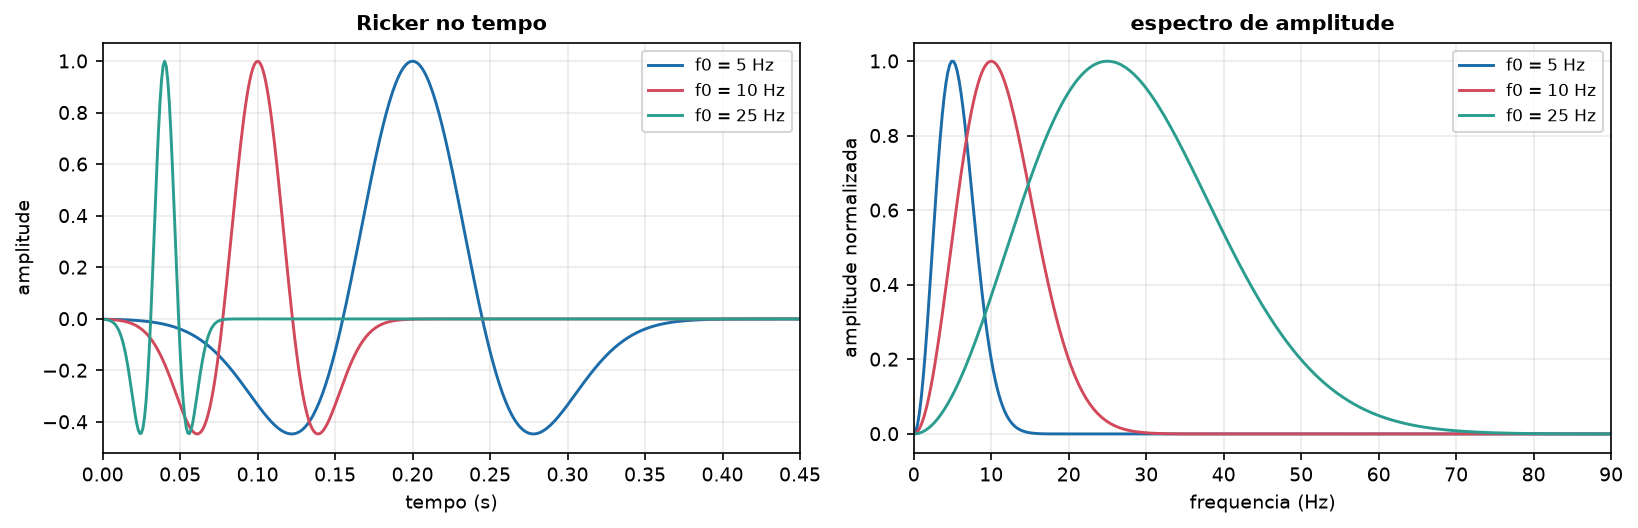
\includegraphics[width=\textwidth]{../saidas/aula01/01_ricker_tempo_frequencia.png}
\caption{Wavelet de Ricker no tempo e na frequência para três valores de
$f_0$. Aumentar $f_0$ estreita o pulso no tempo e alarga o espectro. Gerado
por \arq{aulas/aula01\_regime\_acustico.py}.}
\end{figure}

Medindo numericamente a banda (Tabela gerada pela aula 01):

\begin{center}
\begin{tabular}{@{}rrrrr@{}}
\toprule
$f_0$ (Hz) & pico medido & $f_{\max}$ (--6\,dB) & $/f_0$ & $/f_0$ (--20\,dB) \\
\midrule
5  & 4{,}9  & 8{,}1  & 1{,}61 & 2{,}20 \\
10 & 10{,}0 & 16{,}1 & 1{,}61 & 2{,}20 \\
15 & 14{,}9 & 24{,}4 & 1{,}63 & 2{,}20 \\
25 & 24{,}9 & 40{,}8 & 1{,}63 & 2{,}21 \\
40 & 40{,}0 & 65{,}2 & 1{,}63 & 2{,}21 \\
\bottomrule
\end{tabular}
\end{center}

As duas colunas servem a propósitos diferentes: a --6\,dB ($\approx 1{,}6 f_0$)
é a faixa que move a inversão, e serve para raciocinar sobre \textbf{resolução};
a --20\,dB ($\approx 2{,}2 f_0$) ainda tem energia suficiente para
\emph{dispersar} numericamente, e é a que deve ser usada para dimensionar a
\textbf{malha} --- arredondando para $2{,}5 f_0$ por segurança.

\begin{equation}
\lambda_{\min} = \frac{c_{\min}}{f_{\max}}\ \ (\text{malha: } f_{\max} = 2{,}5 f_0),
\qquad
\text{resolução} \approx \frac{\lambda}{2}\ \ (\text{com } f \approx 1{,}6 f_0).
\end{equation}

% =====================================================================
\chapter{Diferenças finitas: estabilidade e dispersão}
\label{cap:df}

\aula{02}

Estabilidade e dispersão são duas restrições independentes. A primeira decide
se a simulação \emph{roda}; a segunda, se ela está \emph{certa}.

\section{O operador espacial}

A derivada segunda é aproximada por um estêncil centrado:
\begin{equation}
\frac{\partial^{2} f}{\partial x^{2}} \approx
\frac{1}{h^{2}}\left[c_0 f_i + \sum_{k=1}^{N} c_k\,(f_{i+k} + f_{i-k})\right].
\end{equation}

\begin{center}
\begin{tabular}{@{}llp{7.6cm}@{}}
\toprule
\textbf{Ordem} & \textbf{Pontos} & \textbf{Coeficientes $(c_0, c_1, \dots)$} \\
\midrule
O(2) & 3 & $-2$; $+1$ \\
O(4) & 5 & $-5/2$; $+4/3$; $-1/12$ \\
O(8) & 9 & $-205/72$; $+8/5$; $-1/5$; $+8/315$; $-1/560$ \\
\bottomrule
\end{tabular}
\end{center}

A aula 02 verifica numericamente a ordem de convergência em $f(x)=\sin(kx)$.
O erro relativo medido, com o mesmo $h$: $7{,}5\times10^{-3}$ para O(2),
$8{,}9\times10^{-5}$ para O(4) e $2{,}0\times10^{-8}$ para O(8).

Ordem maior não é só ``mais preciso'': é mais preciso \emph{para o mesmo $h$},
o que permite usar $h$ \emph{maior} e economizar memória e tempo.

\section{Estabilidade: a condição CFL}

O esquema \emph{leap-frog} é condicionalmente estável. A análise de von
Neumann leva a
\begin{equation}
C = \frac{c_{\max}\,\Delta t}{\Delta h} \;\le\; C_{\lim},
\qquad
C_{\lim} = \frac{2}{\sqrt{n_{\dim}\bigl(|c_0| + 2\sum_k |c_k|\bigr)}} .
\label{eq:cfl}
\end{equation}

Valores em 2D, medidos pela aula 02: $C_{\lim} = 0{,}7071$ (O2),
$0{,}6124$ (O4), $0{,}5546$ (O8).

\begin{atencao}[Duas leituras contraintuitivas]
\textbf{(a)} Ordem espacial \emph{maior} reduz o $\Delta t$ máximo. O estêncil
mais largo amplifica mais os números de onda altos e a condição aperta. Você
ganha em $\Delta h$ e perde em $\Delta t$.

\textbf{(b)} O limite depende de $c_{\max}$. Uma única célula com velocidade
alta --- sal, basalto, um erro de interpolação --- derruba o $\Delta t$ do
modelo inteiro.
\end{atencao}

A transição não é gradual. A aula 02 mede, com $C_{\lim}=0{,}6124$:
$C = 0{,}306$ e $C = 0{,}551$ ficam estáveis; $C = 0{,}625$ e $C = 0{,}704$
produzem \texttt{NaN}. Não existe ``um pouco instável''. Use sempre uma margem
de 10--20\%.

\section{Dispersão numérica: o erro que parece geologia}

No esquema discreto, a velocidade de fase depende do número de onda. As
componentes de alta frequência viajam com a velocidade errada e o pulso
desenvolve uma cauda oscilatória atrás da frente.

\begin{armadilha}[Por que isso é perigoso]
A cauda dispersiva \emph{parece sinal}: reverberação, camada fina,
\emph{ringing} da fonte. Quem não conhece o efeito interpreta artefato
numérico como geologia --- e, pior, a FWI tenta explicá-lo com estrutura no
modelo.

Teste decisivo: num meio \emph{homogêneo} não há o que refletir. Qualquer
oscilação depois do primeiro pulso é erro numérico.
\end{armadilha}

O controle é o número de pontos por comprimento de onda:
\begin{equation}
G = \frac{\lambda_{\min}}{\Delta h} = \frac{c_{\min}}{f_{\max}\,\Delta h},
\qquad
G \gtrsim \begin{cases} 15\text{--}20 & \text{O(2)}\\ 8\text{--}10 & \text{O(4)}\\ 4\text{--}5 & \text{O(8)}\end{cases}
\end{equation}

\begin{atencao}[A curva espacial \emph{não} é conservadora]
A curva mostrada é a do operador \textbf{espacial} isolado (esquema
semi-discreto, tempo contínuo). A discretização \emph{temporal} acrescenta um
erro próprio, de sinal \textbf{oposto}: o estêncil espacial atrasa a fase, o
\emph{leap-frog} a adianta. Quanto um compensa o outro depende de $C$. Ao longo
de um eixo da malha, o esquema completo obedece a
\[
\frac{4}{\Delta t^{2}}\sin^{2}\!\frac{\omega\Delta t}{2}
 = \frac{c^{2}}{\Delta h^{2}}\,S(k\Delta h),
\qquad
S(\theta) = -\Bigl[c_0 + 2\sum_k c_k\cos(k\theta)\Bigr].
\]

Para O(4) com $G=6$ a curva dá $0{,}9939$. O esquema completo dá $0{,}9980$
com $C=0{,}3$ --- erro menor que o previsto ---, mas $1{,}0081$ com
$C=0{,}551$, que é o $\Delta t$ de \arq{dt\_maximo}: aí o erro real ($0{,}8\%$)
já \emph{supera} o da curva ($0{,}6\%$). Em O(8) o efeito é dramático: com
$G=5$ e $C=0{,}5$ a curva promete $0{,}07\%$ e o esquema entrega $1{,}6\%$,
porque o erro espacial quase sumiu e sobrou o temporal. A verificação 10 de
\arq{verificar\_fisica.py} mede isso no propagador: velocidade de fase
relativa $1{,}0146$, contra $1{,}0160$ da relação completa e $0{,}9993$ da
curva espacial.

Conclusão: perto do limite CFL, e sobretudo em O(8), quem dita a dispersão é
o $\Delta t$. Em modelo heterogêneo isso pesa menos, porque $G$ é calculado com
$c_{\min}$, onde o Courant local é só $C\,c_{\min}/c_{\max}$.
\end{atencao}

\begin{figure}[htbp]
\centering
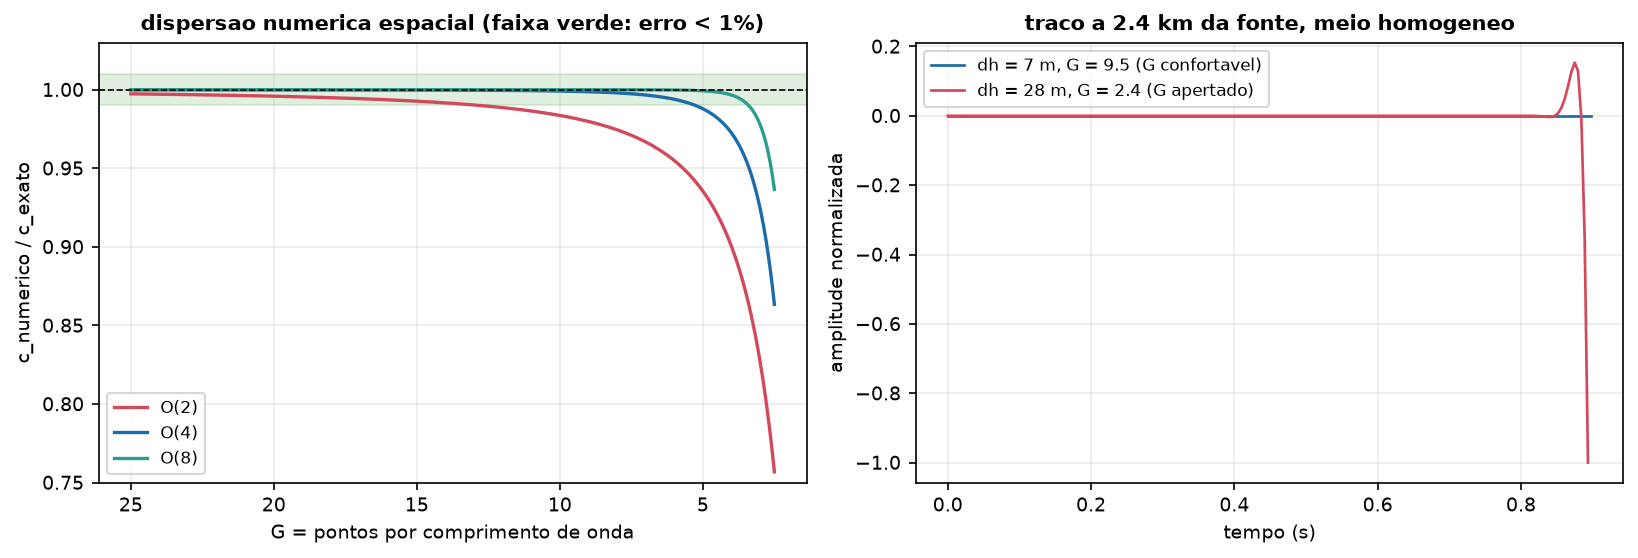
\includegraphics[width=\textwidth]{../saidas/aula02/01_dispersao_numerica.png}
\caption{Esquerda: dispersão do operador \emph{espacial} por ordem (esquema
semi-discreto). Direita: traço a 2{,}3\,km da fonte em meio homogêneo, com
$G=9{,}5$ e $G=2{,}4$. A cauda no traço vermelho não existe na física.}
\end{figure}

\section{Receita de dimensionamento}

\begin{lstlisting}
1. f_max  = 2.5 * f0                       # banda conservadora da Ricker
2. dh     = c_min / (G * f_max)            # G = 8 (O4) ou 5 (O8)
3. dt     = 0.9 * C_lim * dh / c_max       # margem de 10% (O8: reduza C)
4. nt     = tempo_de_registro / dt
5. n_abs >= 0.5 * c_max / (f_min * dh)     # ver Capitulo 4
\end{lstlisting}

\begin{atencao}[O conflito embutido]
$\Delta h$ é ditado por $c_{\min}$ (menor comprimento de onda) e $\Delta t$
por $c_{\max}$ (onda mais rápida). Um modelo com grande contraste --- água a
1500 e sal a 4500 --- é caro dos \emph{dois} lados ao mesmo tempo. É a razão
prática de existirem malhas variáveis e esquemas implícitos.
\end{atencao}

Custo: reduzir $\Delta h$ pela metade quadruplica o número de pontos em 2D
\emph{e} dobra o número de passos (via CFL). Total: $8\times$ em 2D,
$16\times$ em 3D.

% =====================================================================
\chapter{Bordas, superfície livre e aquisição}
\label{cap:bordas}

\aula{03}\quad\aula{04}

\section{Por que as bordas não são detalhe}

O computador só tem um domínio finito; a Terra é praticamente infinita.
Truncar o domínio transforma a borda num espelho.

Em modelagem isso é feio. \textbf{Em FWI é pior}: o resíduo passa a conter
eventos que a física do modelo nunca vai explicar, e o gradiente tenta
explicá-los mexendo na velocidade. Você fabrica estrutura falsa.

\begin{center}
\begin{tabular}{@{}llll@{}}
\toprule
\textbf{Técnica} & \textbf{Como} & \textbf{Custo} & \textbf{Qualidade} \\
\midrule
Truncar          & nada                     & zero  & inaceitável \\
Cerjan (sponge)  & \emph{taper} multiplicativo & baixo & razoável \\
Cond. absorvente & equação unidirecional    & baixo & boa em inc.\ normal \\
CPML             & coordenadas complexas    & médio & excelente \\
\bottomrule
\end{tabular}
\end{center}

\subsection*{Medindo de verdade}

Para medir a reflexão de borda é preciso uma \emph{referência sem borda}:
a mesma simulação num domínio muito maior, onde nada reflete dentro da janela
de tempo. A diferença entre os dois traços é, por construção, só artefato.

\begin{center}
\begin{tabular}{@{}rrrr@{}}
\toprule
\multicolumn{2}{c}{\textbf{Cerjan} (\arq{fwikit})} & \multicolumn{2}{c}{\textbf{CPML} (PyFWI)} \\
$n_{abs}$ & reflexão & $n_{pml}$ & reflexão \\
\midrule
0  & $-6{,}9$ dB  & 0  & $-11{,}2$ dB \\
10 & $-8{,}5$ dB  & 5  & $-20{,}1$ dB \\
20 & $-13{,}3$ dB & 10 & $-51{,}5$ dB \\
30 & $-16{,}5$ dB & 20 & $-69{,}6$ dB \\
45 & $-18{,}4$ dB & 30 & $-77{,}3$ dB \\
\bottomrule
\end{tabular}
\end{center}

Os valores são relativos à onda direta de cada experimento, e as duas
geometrias diferem ($\Delta h$, $f_0$, distância fonte--receptor). A linha
$n=0$ é o espelho --- uma reflexão de 100\%, já atenuada pelo espalhamento
geométrico ---, e a comparação honesta desconta esse valor: o Cerjan com 45
pontos fica $11{,}5$\,dB abaixo do seu espelho ($-18{,}4+6{,}9$); a CPML com
10 pontos fica $40{,}3$\,dB abaixo do dela ($-51{,}5+11{,}2$). A conclusão não
muda, só fica precisa: a CPML com 10 pontos supera com folga o Cerjan com 45.
É por isso que códigos de produção usam CPML.

\begin{pratica}[Por que este curso usa Cerjan mesmo assim]
O \emph{sponge} de Cerjan é um operador \textbf{diagonal}, portanto
auto-adjunto. Isso preserva a validade do teste de gradiente do
Capítulo~\ref{cap:verificacao}
sem exigir que você derive o adjunto de uma CPML.

Há também um ótimo: \emph{taper} fraco demais não absorve, forte demais cria
um degrau de impedância que ele mesmo reflete. O ótimo medido fica em
$\text{fator} \approx 0{,}25/n_{abs}$, e o \arq{fwikit} calibra isso sozinho.
\end{pratica}

\textbf{Dimensionamento:} a moldura precisa de pelo menos meio comprimento de
onda da \emph{menor} frequência usada --- e como a FWI multiescala começa nas
bandas baixas, dimensione por $f_{\min}$, nunca por $f_0$.

\section{Superfície livre: uma escolha física}

No topo há uma decisão que não é numérica:

\textbf{Superfície livre} ($p = 0$ em $z=0$) representa a interface com o ar.
A onda reflete com polaridade invertida, e produz as \emph{múltiplas} de
superfície e o \emph{ghost} --- que são sinais reais do dado.

\textbf{Borda absorvente no topo} representa um meio que continua para cima.
Não é físico, mas elimina múltiplas do sintético.

\begin{armadilha}[O erro de consistência]
Se o dado observado contém múltiplas e o sintético não, esse resíduo inteiro
vai para o gradiente. A FWI tenta reproduzir as múltiplas mexendo na
velocidade. As saídas são duas: modelar a superfície livre, ou remover as
múltiplas do dado antes. Ignorar não é opção.
\end{armadilha}

\section{Aquisição}

A FWI trabalha \emph{sempre} em \emph{shot gathers}, e a razão é conceitual:
$F$ simula um tiro por vez, então o resíduo $F(\mathbf{m}) - \mathbf{d}_{obs}$
tem de ser calculado nessa organização. É também por isso que a FWI não usa
dado empilhado: o empilhamento descarta a dependência com o \emph{offset},
justamente a informação que separa velocidade de profundidade.

\begin{figure}[htbp]
\centering
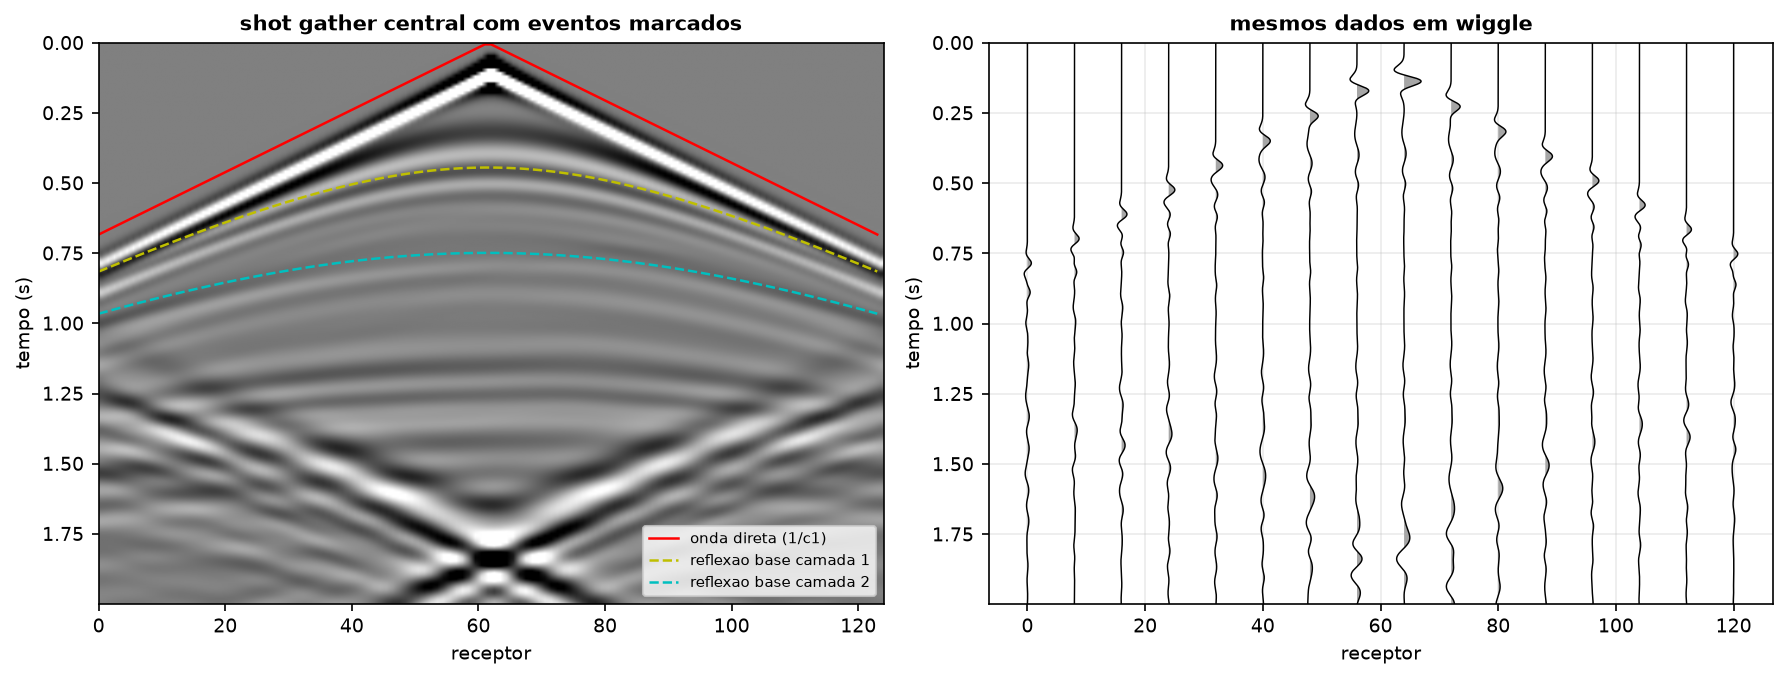
\includegraphics[width=\textwidth]{../saidas/aula04/02_anatomia_shot_gather.png}
\caption{Anatomia de um \emph{shot gather}, com as curvas teóricas
sobrepostas: onda direta (reta), reflexões (hipérboles).}
\end{figure}

\subsection*{Anatomia}
\begin{itemize}[leftmargin=*]
\item \textbf{Onda direta} --- reta de inclinação $1/c_1$, passa pela origem.
Não carrega informação de profundidade; frequentemente é removida.
\item \textbf{Refrações} (\emph{head waves}) --- retas de inclinação $1/c_2$
que cruzam a direta a partir da \textbf{distância de cruzamento}
$x_{cross} = 2h_1\sqrt{(v_2{+}v_1)/(v_2{-}v_1)}$ --- que não se confunde com a
\emph{distância crítica} $2h_1\tan\theta_c$, onde a \emph{head wave} apenas
começa a existir e que é bem menor (1006\,m contra 2291\,m no modelo da
aula 04). Dominam o
\emph{offset} longo e são a fonte mais rica de informação de velocidade de
grande escala.
\item \textbf{Reflexões} --- hipérboles, $t(x)^2 = t_0^2 + x^2/v_{rms}^2$.
A curvatura revela a velocidade média.
\item \textbf{Difrações} --- hipérboles de ápice deslocado.
\end{itemize}

\begin{teoria}[Abertura e profundidade de investigação]
\[
\text{profundidade confiável} \;\approx\; \frac{\text{offset}_{\max}}{3}
\;\text{a}\; \frac{\text{offset}_{\max}}{2}
\]
A razão é geométrica: para separar velocidade de posição é preciso iluminar
cada ponto com \emph{ângulos variados}, e isso exige raios vindo de longe.
\emph{Offset} curto só gera incidência quase normal, que é ambígua --- mais
lento e mais raso produz o mesmo tempo que mais rápido e mais fundo.

\textbf{Consequência prática:} para melhorar a recuperação em profundidade,
aumente o \emph{offset}. Receptores mais densos combatem \emph{aliasing};
mais tiros melhoram razão sinal/ruído; frequência maior melhora resolução ---
mas nenhum deles ilumina mais fundo.
\end{teoria}

\subsection*{Amostragem espacial}
\begin{equation}
\Delta x_{rec} < \frac{c_{ap}}{2 f_{\max}}
\end{equation}
Acima disso há \emph{aliasing} espacial: eventos inclinados deixam de ser
contínuos. Em FWI isso é especialmente perverso, porque a inversão tenta
explicar o padrão serrilhado com estrutura no modelo.

\subsection*{Ruído}
A FWI tolera bem ruído \emph{aleatório}: ele não soma coerentemente no
gradiente quando se empilham muitos tiros. O que ela \emph{não} tolera é ruído
\textbf{coerente} e erro de modelagem sistemático --- esses somam em fase e
viram estrutura.

% =====================================================================
\part*{\centering\color{azulfwi} Parte II --- PyFWI}
\addcontentsline{toc}{part}{Parte II --- PyFWI}

\chapter{PyFWI na prática}
\label{cap:pyfwi}

\aula{05}

\section{A anatomia de um script}

Todo script de PyFWI tem quatro blocos. Vale memorizar, porque a documentação
do pacote é escassa.

\begin{lstlisting}
# 1. PARAMETROS -- um dicionario unico
inpa = {'ns':1, 'sdo':4, 'fdom':20, 'dh':7, 'dt':0.0005, 't':0.5,
        'npml':20, 'pmlR':1e-5, 'pml_dir':2, 'acq_type':1, 'device':0}

# 2. MODELO -- dicionario com 'vp', 'vs', 'rho'
model = md.ModelGenerator('louboutin')()

# 3. AQUISICAO -- posicoes em METROS
src_loc, rec_loc = acq.surface_seismic(ns, rec_dis, offsetx, dh, sdo)
src = acq.Source(src_loc, dh, dt);  src.Ricker(fdom)

# 4. PROPAGADOR
W = wave.WavePropagator(inpa, src, rec_loc, (nz,nx),
                        n_well_rec=0, chpr=0, components=0)
d = W.forward_modeling(model, show=False)
\end{lstlisting}

\begin{armadilha}[Três armadilhas que custam tempo]
\textbf{1.} Posições de fonte e receptor são dadas em \textbf{metros}, não em
índices de malha.

\textbf{2.} \texttt{inpa['sdo']} é a ordem espacial \emph{real} (4 ou 8), mas
internamente o código faz \texttt{self.sdo = sdo/2}.

\textbf{3.} \texttt{inpa['acq\_type']} seleciona o \emph{kernel} e o mapeamento
de receptores: \textbf{0 = \emph{crosswell}}, \textbf{1 = superfície},
\textbf{2 = ambos}. Os três são válidos --- e é justamente por isso que o
descuido é perigoso: se o valor não casar com a geometria que você montou, o
código \emph{não} levanta erro, mapeia os receptores por outro caminho e
devolve um sismograma plausível e errado. Veja a Seção \ref{sec:validacao}.
\end{armadilha}

\section{O parâmetro \texttt{components}}

\begin{center}
\begin{tabular}{@{}clp{7cm}@{}}
\toprule
\textbf{\texttt{components}} & \textbf{Campos} & \textbf{Interpretação} \\
\midrule
0 & \texttt{taux}, \texttt{tauz} (média) & $(\sigma_{xx}+\sigma_{zz})/2 = -p$ --- \textbf{pressão com o sinal trocado} \\
1 & \texttt{taux} & só a tensão normal em $x$ \\
2 & \texttt{vx}, \texttt{vz} & velocidade de partícula (geofone) \\
3 & tensor de tensões completo & para inspecionar a física \\
4 & tudo & \\
\bottomrule
\end{tabular}
\end{center}

\begin{armadilha}[O sinal de \texttt{components=0}]
O PyFWI devolve a \emph{média das tensões normais}, não a pressão:
\texttt{acquisition.seismic\_section} faz literalmente
\texttt{(taux + tauz)/2}. Como \texttt{taux}$\,=\sigma_{xx}$ na convenção de
tração positiva do \emph{kernel}, isso é $(\sigma_{xx}+\sigma_{zz})/2 = -p$
pela definição \eqref{eq:pressao}. Para ler pressão, \textbf{inverta o sinal}.

Num L2 puramente sintético a polaridade se cancela e o erro passa
despercebido; ao comparar com outro código --- ou com dado real de hidrofone
--- ela aparece como correlação negativa.
\end{armadilha}

\section{A prova numérica do regime acústico}

O Capítulo \ref{cap:acustico} afirmou que a aproximação acústica é a hipótese
$\mu = 0$, e que dela decorre um tensor de tensões isotrópico. Podemos
\emph{comprovar} isso no próprio PyFWI, que resolve o sistema elástico
completo. O experimento: a mesma simulação duas vezes, mudando só $v_s$.

\begin{center}
\begin{tabular}{@{}lcc@{}}
\toprule
\textbf{Caso} & $\|\sigma_{xx}-\sigma_{zz}\| / \|\sigma_{xx}\|$ & $\|\sigma_{xz}\| / \|\sigma_{xx}\|$ \\
\midrule
Elástico ($v_s = v_p/\sqrt{3}$) & $3{,}20\times10^{-1}$ & $3{,}91\times10^{-1}$ \\
Acústico ($v_s = 0$)            & $4{,}48\times10^{-7}$ & $\mathbf{0{,}0}$ \\
\bottomrule
\end{tabular}
\end{center}

\begin{teoria}[Leia estes números]
No caso \textbf{elástico}, $\sigma_{xx}$ e $\sigma_{zz}$ diferem em $\sim$32\%
e $\sigma_{xz}$ vale $\sim$39\% de $\sigma_{xx}$: existe cisalhamento de
verdade.

No caso \textbf{acústico}, $\sigma_{xx}-\sigma_{zz}$ cai para $10^{-7}$ ---
zero até a precisão de \texttt{float32} --- e $\sigma_{xz}$ dá
\textbf{exatamente} $0{,}0$, porque $\mu$ multiplica o termo inteiro.

É a demonstração numérica de \eqref{eq:hipotese} e \eqref{eq:pressao}.
\textbf{O PyFWI não tem um solver acústico separado}: ele tem um solver
elástico, e o regime acústico se obtém zerando $v_s$ \emph{no modelo} ---
não apenas pedindo \texttt{components=0}, que só escolhe o que é gravado.
\end{teoria}

\begin{figure}[htbp]
\centering
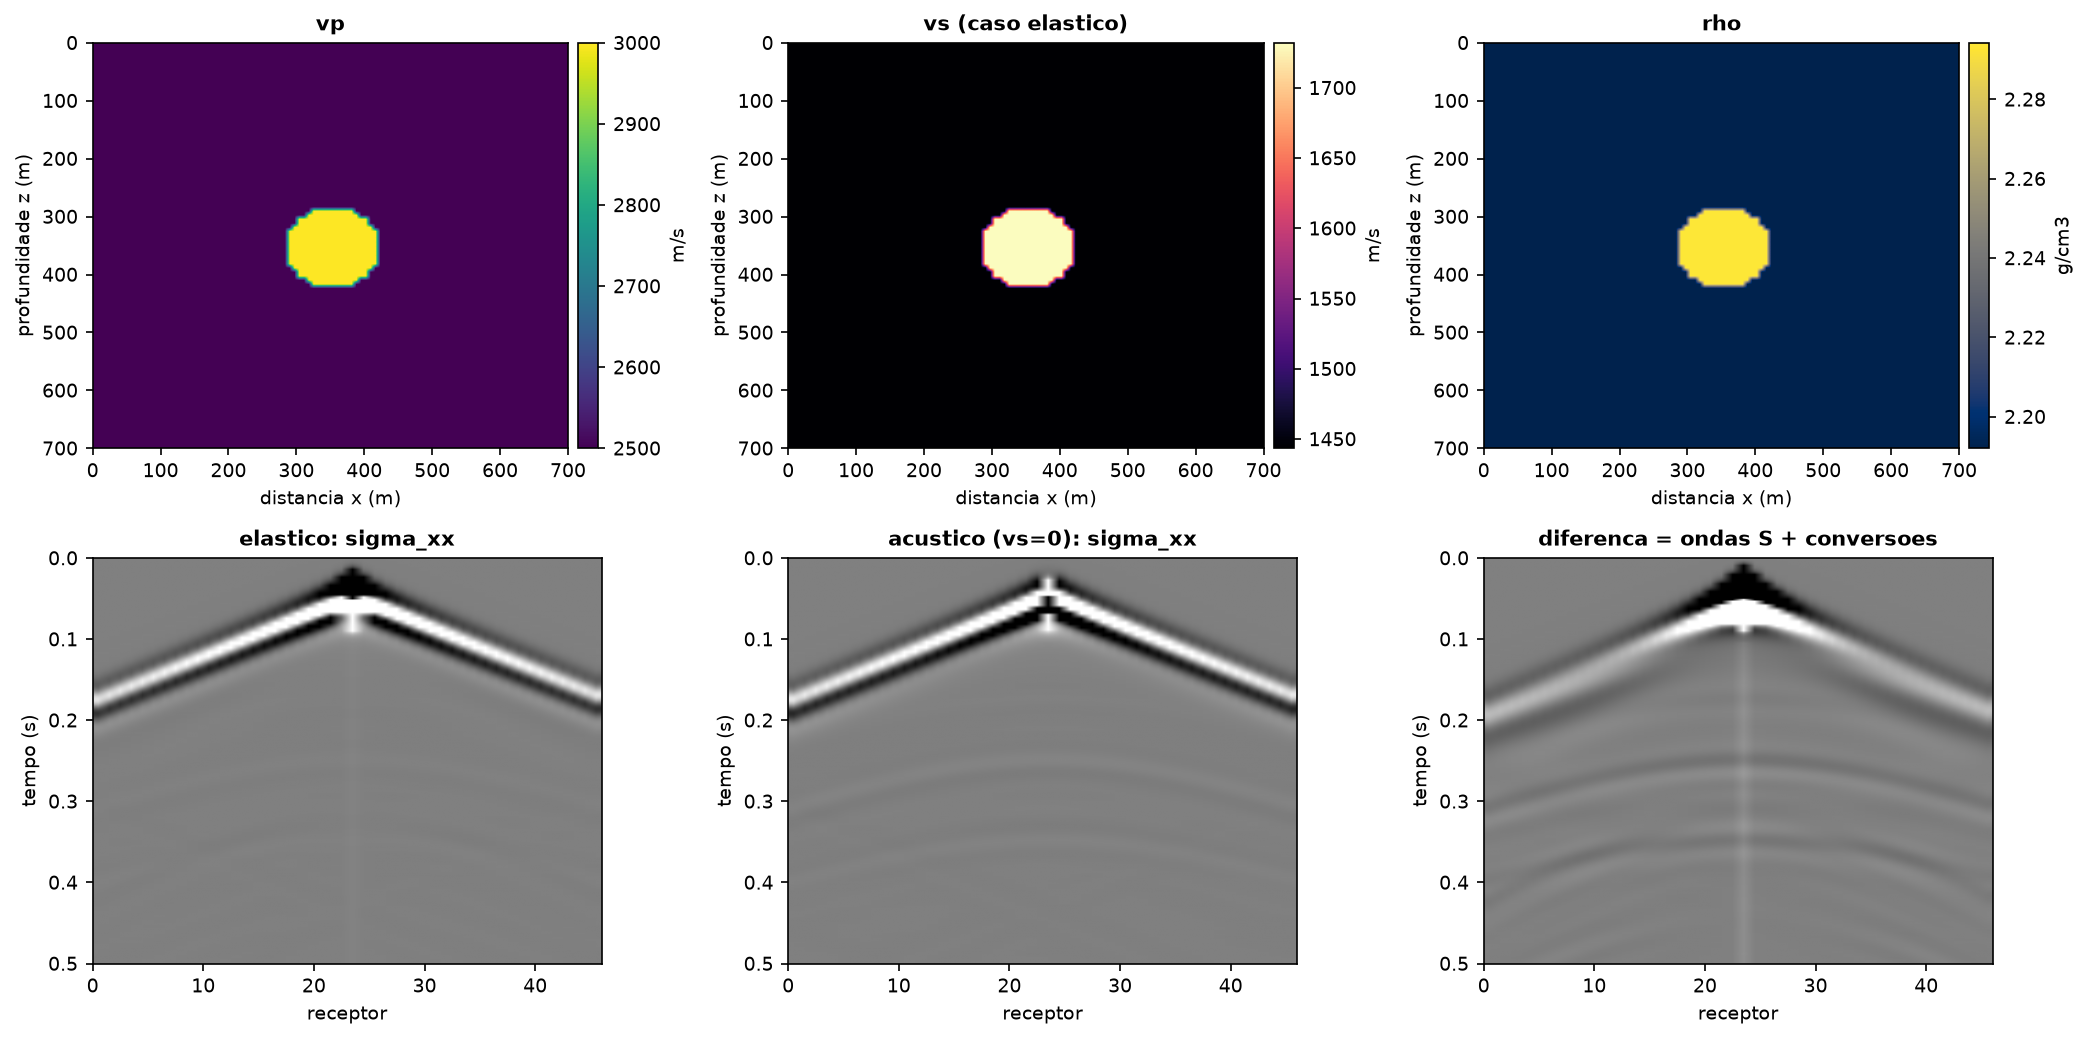
\includegraphics[width=\textwidth]{../saidas/aula05/01_prova_regime_acustico.png}
\caption{Prova do regime acústico. Painel inferior direito: a diferença entre
elástico e acústico são as ondas S e conversões P--S --- com norma comparável
à do próprio dado.}
\end{figure}

\section{Por que as formas diferem (e não é erro de nenhum dos dois)}

A cinemática bate, mas sobrepondo os traços a \emph{forma} do pulso difere. A
explicação é exata e já está no Capítulo \ref{cap:acustico}: as duas
formulações têm wavelets efetivas que diferem por uma derivada temporal.

Medindo a correlação média sobre todos os receptores:

\begin{center}
\begin{tabular}{@{}lr@{}}
\toprule
\textbf{Comparação} & \textbf{Correlação média} \\
\midrule
traços como saem dos dois códigos & $+0{,}1235$ \\
derivando no tempo o traço do \arq{fwikit} & $\mathbf{+0{,}8501}$ \\
\bottomrule
\end{tabular}
\end{center}

Sem ajuste e sem parâmetro livre: é exatamente a relação prevista. Os dois
códigos estão certos; o que diferia era a \textbf{convenção de fonte}, não a
física.

\begin{atencao}[Por que a correlação sai \emph{positiva}]
Vale fechar a conta dos sinais, porque ela envolve duas inversões que se
cancelam. O traço do PyFWI é $(\sigma_{xx}+\sigma_{zz})/2 = -p$ --- primeira
inversão. E a fonte explosiva do PyFWI (\texttt{src\_type=0}) soma
$+w(t)$ às \emph{tensões} normais, o que em pressão é $-w(t)$, enquanto o
\arq{fwikit} soma $+w(t)$ direto na pressão --- segunda inversão. As duas se
anulam, e a correlação com a derivada temporal sai $+0{,}85$ em vez de
$-0{,}85$.

A lição não muda: \emph{conte os sinais explicitamente}. Aqui eles se
cancelaram por sorte; uma comparação em que sobrasse um sinal seria lida como
``os códigos discordam'' quando o que discorda é a convenção.
\end{atencao}

\begin{pratica}[As perguntas certas ao comparar dois códigos de onda]
Antes de suspeitar da física, verifique a convenção de fonte:
\begin{itemize}[leftmargin=*]
\item a formulação é de primeira ou de segunda ordem?
\item a fonte entra na pressão, na tensão ou na velocidade de partícula?
\item há divisão por $\Delta h^{2}$ (discretização da delta)?
\end{itemize}
Cada uma dessas escolhas muda a wavelet efetiva --- e nenhuma delas aparece no
sismograma com uma etiqueta.
\end{pratica}

\section{Validação cruzada: como esta comparação achou um bug}
\label{sec:validacao}

\begin{armadilha}[Um caso real, ocorrido na montagem deste curso]
A comparação entre o PyFWI e o \arq{fwikit} falhou: os dois códigos
discordavam em 159\,ms, e o \emph{gather} do PyFWI \textbf{não tinha ápice} ---
a curva subia monotonicamente do receptor 0 ao 45, como se a fonte estivesse
fora do arranjo.

A causa era \texttt{acq\_type = 0} com uma geometria de \emph{superfície}. O
valor 0 não é inválido --- é o código de \emph{crosswell}
(\texttt{acquisition.acq\_parameters}: 0 = crosswell, 1 = superfície,
2 = ambos). O PyFWI então compilou o \emph{kernel} de poço e mapeou os
receptores ao longo de uma vertical, sobre posições que na verdade eram uma
linha horizontal. Nenhum erro é levantado: as duas configurações são legítimas,
só não combinavam entre si.

Duas lições, e a segunda vale mais:
\begin{enumerate}
\item Em aquisição de superfície, \texttt{acq\_type = 1}. Sempre --- e confira
que ele casa com a função que gerou as posições
(\texttt{surface\_seismic} $\leftrightarrow$ 1,
\texttt{crosswell} $\leftrightarrow$ 0).
\item \textbf{Um dado sintético errado quase nunca vem com aviso. Ele vem
bonito.} A defesa barata é comparar com uma implementação independente e
checar se a física elementar aparece --- neste caso, se o ápice da
\emph{moveout} cai sobre a fonte. Faça isso \emph{antes} de rodar qualquer
inversão.
\end{enumerate}
\end{armadilha}

Após a correção, a comparação passa: ápice no receptor 22 ($x=336$\,m) contra
23 ($x=350$\,m), com a fonte em 350\,m, e erro rms das primeiras chegadas de
4{,}4\,ms.

\textbf{O que comparar:} escolha a \textbf{cinemática}, não a forma do traço.
Os dois códigos resolvem discretizações diferentes (velocity--stress
intercalado com CPML e densidade variável \emph{versus} pressão colocalizada
com Cerjan e densidade constante). Amplitude e fase fina \emph{vão} diferir,
e isso não é erro. Tempo de trânsito é propriedade da física, não da
discretização.

% =====================================================================
\chapter{PyFWI por dentro: parâmetros e custo}

\aula{06}

\section{Referência do dicionário \texttt{inpa}}

Levantada lendo o código-fonte, porque não existe na documentação.

\begin{center}
\small
\begin{longtable}{@{}llp{8.2cm}@{}}
\toprule
\textbf{Chave} & \textbf{Obrigatória} & \textbf{O que faz} \\
\midrule
\endhead
\texttt{dh} & sim & espaçamento da malha (m) \\
\texttt{dt} & sim & passo de tempo pedido (veja o reescalonamento) \\
\texttt{t} & sim & duração do registro (s) \\
\texttt{sdo} & não ($=4$) & ordem espacial \emph{real}: 4 ou 8; omitir equivale a 4 \\
\texttt{npml} & não (0) & espessura da CPML em pontos \\
\texttt{pmlR} & com \texttt{npml} & coef.\ de reflexão teórico (ex.\ 1e-5) \\
\texttt{pml\_dir} & com \texttt{npml} & 0 = só $z$; 1 = só $x$; 2 = ambas; 3 = ambas sem o topo \\
\texttt{acq\_type} & não (1) & 0 = \emph{crosswell}; 1 = superfície; 2 = ambos \\
\texttt{device} & não (0) & índice do dispositivo OpenCL \\
\texttt{seimogram\_shape} & não ('2d') & '2d' $\to (n_t, n_r n_s)$; '3d' $\to (n_t,n_r,n_s)$ \\
\texttt{g\_smooth} & não (0) & $\sigma$ da suavização gaussiana do gradiente \\
\texttt{energy\_balancing} & não (False) & normaliza pela iluminação \\
\texttt{cost\_function\_type} & não ('l2') & funcional de erro \\
\texttt{grad\_coeff} & não ([1,1,1]) & pesos de $v_p$, $v_s$, $\rho$ \\
\texttt{tv} / \texttt{tikhonov} & não & dicionários de regularização \\
\texttt{prior\_model} & não & modelo a priori \\
\bottomrule
\end{longtable}
\end{center}

\begin{armadilha}[Três entradas fáceis de documentar errado]
\textbf{\texttt{pml\_dir} é invertido em relação à intuição.} No código, o
valor 0 \emph{zera} a PML em $x$ (sobra só $z$) e o valor 1 zera a PML em $z$
(sobra só $x$) --- o número indica a direção que você \emph{desliga}. O valor 3
mantém as duas mas remove a PML do \emph{topo}, que é como se modela superfície
livre.

\textbf{\texttt{sd} não é passo de otimização.} É um peso que multiplica os
dados \emph{calculados} (\texttt{prepare\_residual(d\_est, sd)}), enquanto os
observados entram com peso 1. Deixe em $1{,}0$.

\textbf{Omitir \texttt{sdo} não dá ordem 2.} O código faz
\texttt{self.sdo = sdo/2} e usa 2 como padrão interno, o que corresponde à
ordem espacial \emph{real} 4.
\end{armadilha}

\begin{armadilha}[O \emph{typo} que o pacote carrega]
A chave é \texttt{seimogram\_shape}, não \texttt{seismogram\_shape}. Escrever
\emph{certo} faz o PyFWI ignorar a chave em silêncio. Erros assim são a razão
de você \textbf{sempre} conferir \texttt{d.shape} depois da modelagem.
\end{armadilha}

\section{O reescalonamento automático de \texttt{dt}}

O PyFWI não usa o $\Delta t$ que você pede:
\begin{lstlisting}
self.dt_scale = np.ceil(inpa['dt'] / 0.0006)
self.dt       = inpa['dt'] / self.dt_scale
\end{lstlisting}

Existe um teto rígido de 0{,}6\,ms no passo interno. Pedir
$\Delta t = 2$\,ms faz o PyFWI subdividir em 4 passos de 0{,}5\,ms.

\begin{pratica}[Três consequências]
\begin{itemize}[leftmargin=*]
\item Pedir $\Delta t$ grande \textbf{não} economiza computação --- só reduz o
tamanho do sismograma de saída.
\item O teto é calibrado para $\Delta h$ de poucos metros. Com $\Delta h$
grande (25--50\,m), esse $\Delta t$ fica desnecessariamente pequeno.
\item O PyFWI \textbf{não} verifica CFL contra o seu $c_{\max}$. Essa conta
continua sendo sua.
\end{itemize}
\end{pratica}

\section{Checkpointing: o compromisso central}

Para o gradiente adjunto é preciso correlacionar o campo direto com o
adjunto, em cada ponto e cada instante. Mas o direto avança e o adjunto
retrocede.

\begin{center}
\begin{tabular}{@{}llll@{}}
\toprule
\textbf{Estratégia} & \textbf{Memória} & \textbf{Computação} & \textbf{Uso} \\
\midrule
Guardar tudo    & $n_t n_z n_x$    & 1 modelagem   & 2D pequeno (\arq{fwikit}) \\
Recomputar      & 1 campo          & $\sim n_t$    & nunca \\
Checkpointing   & $n_{chk} n_z n_x$& $\sim 2$      & o padrão (\texttt{chpr}) \\
Reversão de campo & contorno       & 2             & se não há atenuação \\
\bottomrule
\end{tabular}
\end{center}

\begin{atencao}[Em 3D isso deixa de ser acadêmico]
Um modelo $500\times500\times300$ com $n_t = 5000$ exigiria \textbf{1{,}5\,TB
por tiro} para guardar tudo. Por isso todo código de FWI 3D usa
checkpointing.

Detalhe pouco mencionado: a \emph{reversão de campo} exige que o operador seja
reversível no tempo. Sem atenuação, é. \emph{Com} atenuação, não --- reverter
um meio dissipativo amplifica ruído exponencialmente.
\end{atencao}

\section{A conta que evita surpresas}
\begin{equation}
\text{custo} \;\approx\; n_{iter} \times n_{freq} \times n_{tiros}
\times 2 \times \text{custo}_{\text{modelagem}}
\end{equation}
O fator 2 é direto + adjunto; a busca linear costuma dobrar de novo.

\begin{pratica}[As duas alavancas que mudam ordens de grandeza]
\textbf{Paralelismo por tiro.} Os tiros são independentes --- o gradiente é
uma \emph{soma} sobre eles. É paralelismo trivial e é a primeira coisa a
fazer.

\textbf{Subconjunto aleatório de tiros} por iteração. Em vez de 200 tiros, use
20 sorteados a cada iteração. O gradiente fica ruidoso, mas a direção média
está certa e o custo cai $10\times$.
\end{pratica}

% =====================================================================
\part*{\centering\color{azulfwi} Parte III --- O problema inverso}
\addcontentsline{toc}{part}{Parte III --- O problema inverso}

\chapter{Função objetivo e cycle skipping}
\label{cap:inverso}

\aula{07}

\section{Formulação}

Com $F$ o operador direto e $\mathbf{m}$ o vetor de parâmetros:
\begin{align}
\mathbf{d}_{calc} &= F(\mathbf{m}), \\
\mathbf{r}(\mathbf{m}) &= F(\mathbf{m}) - \mathbf{d}_{obs}, \\
J(\mathbf{m}) &= \tfrac{1}{2}\|\mathbf{r}\|^{2}
 = \tfrac{1}{2}\sum_{s}\sum_{r}\int_{0}^{T} r^{2}(x_r,t;s)\,dt .
\end{align}

A solução iterativa tem sempre a mesma forma:
\begin{equation}
\mathbf{m}_{k+1} = \mathbf{m}_{k} + \alpha_k \mathbf{d}_k ,
\label{eq:iteracao}
\end{equation}
com $\mathbf{d}_k$ a direção de busca (construída a partir do gradiente) e
$\alpha_k$ o passo, obtido por busca linear.

\begin{teoria}[Três propriedades de $J$]
\textbf{Não linear.} $F$ depende de $\mathbf{m}$ de forma não linear --- a
velocidade aparece dentro do operador de onda, e o tempo de trânsito depende
dela de maneira integral. Não há solução fechada.

\textbf{Não convexa.} Existem mínimos locais, muitos. Um otimizador local
converge para o mais próximo do ponto de partida.

\textbf{Mal posta.} Partes do modelo não são vistas pelos dados. Ali o
gradiente é $\approx 0$ e o modelo fica onde estava --- ou é preenchido por
artefatos vindos da regularização.
\end{teoria}

\section{Vendo a não convexidade}

Num meio homogêneo com um único parâmetro $c$, é possível varrer $c$ e
desenhar $J(c)$ inteiro --- coisa impossível com $10^6$ parâmetros.

\begin{figure}[htbp]
\centering
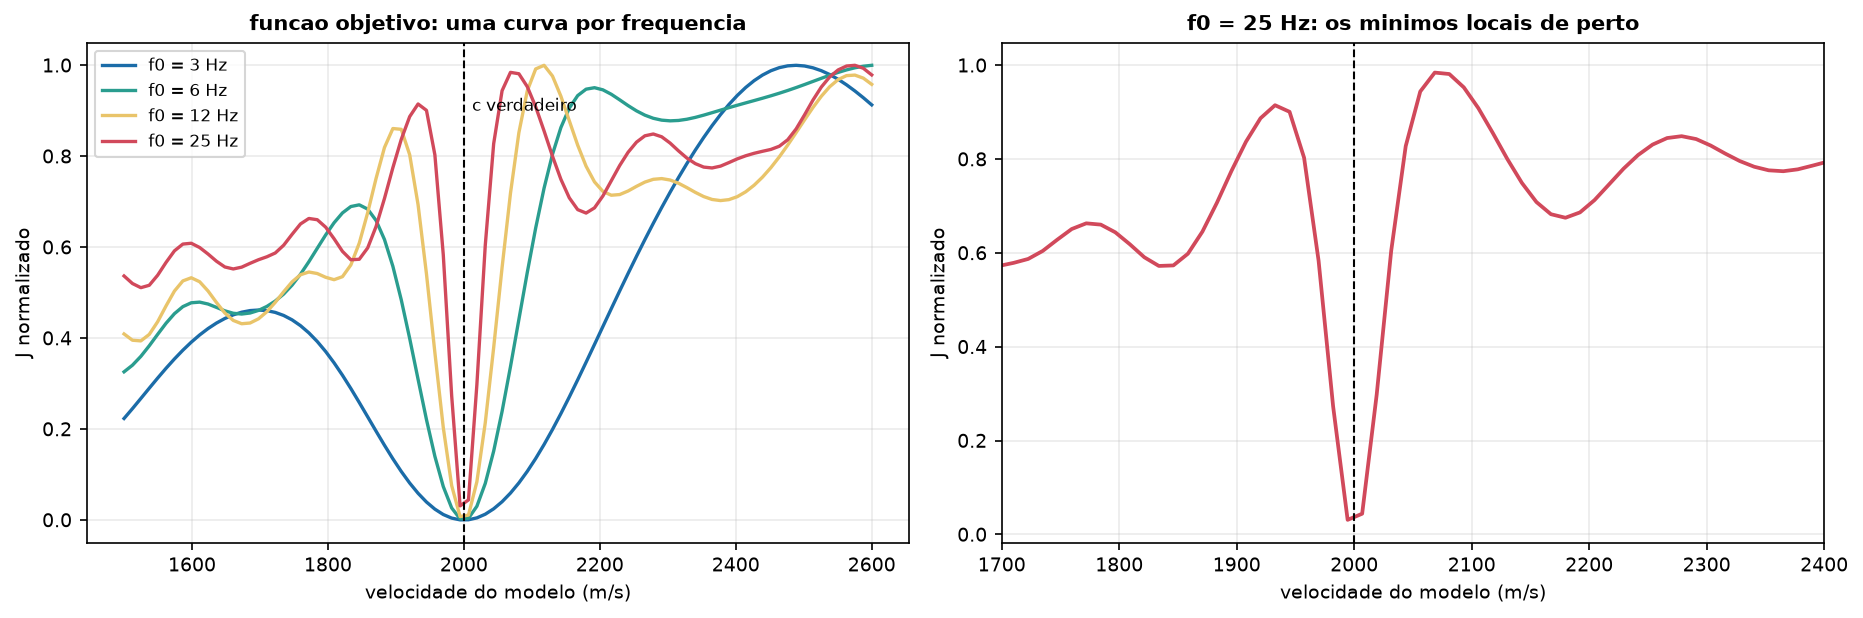
\includegraphics[width=\textwidth]{../saidas/aula07/01_funcao_objetivo.png}
\caption{$J(c)$ para quatro frequências, meio homogêneo, $c$ verdadeiro
$=2000$\,m/s. Em baixa frequência há um único mínimo largo; em alta
frequência, um vale estreito cercado de mínimos locais.}
\end{figure}

Essa figura contém a ideia mais importante do curso. Em \textbf{baixa}
frequência a curva é larga e tem um único mínimo: qualquer modelo inicial
dentro de uma faixa generosa converge. Em \textbf{alta} frequência a curva
vira um vale estreito cercado de mínimos locais.

\section{Cycle skipping: a explicação física}

A razão é puramente de \emph{fase}. Se o modelo está errado, o evento
sintético chega deslocado de $\delta t$ em relação ao observado. Para um pulso
aproximadamente harmônico de período $T$:

\begin{itemize}[leftmargin=*]
\item $|\delta t| < T/2$: sintético e observado ainda se sobrepõem no
\emph{mesmo} ciclo. O resíduo aponta na direção certa e a inversão corrige.
\item $|\delta t| > T/2$: o sintético se alinha com o ciclo \emph{vizinho}. O
resíduo diminui ao empurrar o modelo para o lado \emph{errado}.
\end{itemize}

\begin{equation}
\boxed{\;|\delta t| < \frac{T}{2} = \frac{1}{2f}\;}
\label{eq:meiociclo}
\end{equation}

Para um percurso de comprimento $L$, $\delta t = L(1/c_{ini} - 1/c_{verd})$, e
o critério vira uma tolerância explícita no erro de velocidade:
\begin{equation}
|\delta c| < \frac{c^{2}}{2 f L}.
\label{eq:tolerancia}
\end{equation}

\begin{center}
\begin{tabular}{@{}rrrr@{}}
\toprule
$f$ (Hz) & $T/2$ (ms) & $|\delta c|_{\max}$ (m/s) & em \% \\
\midrule
2  & 250{,}0 & 667 & 33{,}3 \\
3  & 166{,}7 & 444 & 22{,}2 \\
5  & 100{,}0 & 267 & 13{,}3 \\
10 & 50{,}0  & 133 & 6{,}7 \\
20 & 25{,}0  & 67  & 3{,}3 \\
40 & 12{,}5  & 33  & 1{,}7 \\
\bottomrule
\end{tabular}
\end{center}
{\small ($L = 1500$\,m, $c = 2000$\,m/s)}

A 2\,Hz você pode errar 33\% e ainda convergir. A 40\,Hz precisa começar com
menos de 2\% de erro --- ou seja, precisaria já saber a resposta.

\subsection*{Validação numérica do critério}

A aula 07 mede o \emph{vale de atração} de cada frequência --- o conjunto de
velocidades iniciais que converge para o mínimo certo --- e compara com
\eqref{eq:tolerancia}:

\begin{center}
\begin{tabular}{@{}rrrr@{}}
\toprule
$f_0$ (Hz) & vale medido (m/s) & semilargura prevista & semilargura medida \\
\midrule
3{,}0  & 1710 a 2489 & 422 & 389 \\
6{,}0  & 1858 a 2192 & 211 & 167 \\
12{,}0 & 1908 a 2118 & 105 & 105 \\
25{,}0 & 1945 a 2069 & 51  & 62 \\
\bottomrule
\end{tabular}
\end{center}

Uma conta de meia linha reproduz a largura medida e a dependência $1/f$ ao
longo de uma faixa de $8\times$ em frequência.

\begin{pratica}[Use isso antes de rodar]
Estime a frequência mais alta com que pode \emph{começar}, dada a incerteza
do seu modelo inicial. Se a tomografia tem 5\% de erro e o percurso típico é
2\,km, com $c = 2000$\,m/s:
\[
\delta c = 100\ \text{m/s} \;\Rightarrow\;
f_{\max} = \frac{c^{2}}{2\,\delta c\,L} = 10\ \text{Hz}.
\]
Começar acima disso é desperdício de tempo de máquina.
\end{pratica}

\section{A estratégia multiescala}

Daí decorre, sem mais nenhuma hipótese, a receita de Bunks \emph{et al.}
(1995): inverta primeiro nas frequências baixas, onde o vale é largo; use o
resultado como modelo inicial da banda seguinte; repita subindo. Multiescala
não é um truque numérico --- é a consequência direta de \eqref{eq:meiociclo}.

\section{O modelo inicial}

O modelo inicial não precisa ser bonito nem detalhado. Precisa de uma coisa:
estar dentro do vale de atração da \emph{menor} frequência utilizável. Isso
significa acertar os \emph{grandes} comprimentos de onda, não os detalhes.

\begin{armadilha}[Sobre testes sintéticos]
Usar o modelo verdadeiro suavizado como inicial --- o que
\texttt{ModelGenerator(...)(smoothing=1)} faz --- é um teste \textbf{generoso}:
ele já começa dentro do vale por construção.

Não está errado usá-lo para validar código. Mas não confunda isso com avaliar
a \emph{robustez} do método. Para isso, degrade o modelo inicial de propósito
e descubra onde ele quebra. Um experimento que só funciona com inicial
privilegiado diz muito pouco sobre dado real.
\end{armadilha}

\section{Além do L2}

Como o problema do L2 é de fase, boa parte da pesquisa consiste em trocar o
funcional:

\begin{center}
\begin{tabular}{@{}lll@{}}
\toprule
\textbf{Funcional} & \textbf{Ideia} & \textbf{Preço} \\
\midrule
L2 clássico & diferença amostra a amostra & cycle skipping \\
Envoltória & compara envoltórias & perde resolução \\
Correlação cruzada & penaliza o deslocamento & precisa janelar \\
Transporte ótimo & distância entre ``massas'' & custo alto \\
Adaptativa (AWI) & penaliza o filtro de casamento & mais parâmetros \\
\bottomrule
\end{tabular}
\end{center}

\begin{pratica}[Ordem de prioridade quando a FWI não converge]
1. Baixe a frequência inicial. \quad 2. Melhore o modelo inicial. \quad
3. \emph{Só então} troque o funcional.

Trocar o funcional é a solução mais cara e a que mais introduz parâmetros
novos. Ela resolve casos em que 1 e 2 já foram esgotados.
\end{pratica}

% =====================================================================
\chapter{O método do estado adjunto}
\label{cap:adjunto}

\aula{08}

\section{Por que não diferenças finitas}

O custo da abordagem ingênua é $N$ modelagens \emph{por iteração}:

\begin{center}
\begin{tabular}{@{}lrrr@{}}
\toprule
\textbf{Modelo} & $N$ & \textbf{modelagens/iter} & \textbf{tempo (a 0{,}4\,s cada)} \\
\midrule
$100\times100$   & 10\,000     & 10\,000     & 1{,}1 horas \\
$200\times400$   & 80\,000     & 80\,000     & 8{,}9 horas \\
$500\times1000$  & 500\,000    & 500\,000    & 2{,}3 dias \\
3D $300^{3}$     & 27\,000\,000& 27\,000\,000& 125 dias \\
\bottomrule
\end{tabular}
\end{center}

Nem em 2D pequeno isso é aceitável.

\section{A derivação}

Trabalhamos com $m(\mathbf{x}) = 1/c(\mathbf{x})^{2}$, porque a equação é
linear nele. O problema direto, como restrição:
\begin{equation}
\mathcal{F}(p,m) \;\equiv\; m\,\frac{\partial^{2}p}{\partial t^{2}}
 - \nabla^{2}p - s \;=\; 0 .
\end{equation}

\subsection*{Passo 1 --- Lagrangiano}

A restrição vale para todo $\mathbf{x}$ e todo $t$; introduzimos um
multiplicador $\lambda(\mathbf{x},t)$:
\begin{equation}
\mathcal{L} = J + \int_{\Omega}\!\!\int_{0}^{T}
\lambda\left[m\,\partial_{tt}p - \nabla^{2}p - s\right] dt\,d\mathbf{x}.
\end{equation}
Como a restrição é satisfeita pela solução, $\mathcal{L} = J$ --- e podemos
derivar $\mathcal{L}$ em vez de $J$, com a vantagem de podermos
\emph{escolher} $\lambda$ para matar o termo difícil.

\subsection*{Passo 2 --- variação em relação a $p$}

Integrando por partes duas vezes no tempo (as derivadas passam de $p$ para
$\lambda$) e duas vezes no espaço (o laplaciano é auto-adjunto):
\begin{equation}
\frac{\delta\mathcal{L}}{\delta p}
 = \left[m\,\partial_{tt}\lambda - \nabla^{2}\lambda\right]
 + \sum_{r} r(t)\,\delta(\mathbf{x}-\mathbf{x}_r).
\end{equation}

\subsection*{Passo 3 --- escolher $\lambda$}

Exigindo $\delta\mathcal{L}/\delta p = 0$, o termo que dependia da variação de
$p$ desaparece. Isso \emph{define} a equação adjunta:
\begin{equation}
\boxed{\;
m\,\frac{\partial^{2}\lambda}{\partial t^{2}} - \nabla^{2}\lambda
 = -\sum_{r} r(t)\,\delta(\mathbf{x}-\mathbf{x}_r)\;}
\label{eq:adjunta}
\end{equation}
com condições \textbf{finais} nulas: $\lambda = \partial_t\lambda = 0$ em
$t = T$.

\begin{teoria}[Leia a equação adjunta]
É a \emph{mesma} equação de onda do problema direto. Mudam duas coisas:

\textbf{(1)} A fonte não é mais a wavelet no ponto de tiro: é o
\textbf{resíduo}, com sinal trocado, injetado em \emph{todos} os receptores ao
mesmo tempo. Cada receptor vira uma fonte.

\textbf{(2)} As condições são \emph{finais}: resolve-se de trás para frente.

Interpretação física: você pega o erro que sobrou nos receptores e o joga de
volta para dentro da Terra, para ver de onde ele veio.

Como a equação acústica sem atenuação é \textbf{auto-adjunta} (invariante por
reversão temporal), basta rodar o mesmo propagador ao contrário. Em meios
dissipativos essa simetria se perde.
\end{teoria}

\subsection*{Passo 4 --- variação em relação a $m$}

Com $\lambda$ escolhido, o único termo que sobra é
\begin{equation}
\boxed{\;
\frac{\partial J}{\partial m}(\mathbf{x})
 = \int_{0}^{T} \lambda(\mathbf{x},t)\,
   \frac{\partial^{2}p}{\partial t^{2}}(\mathbf{x},t)\; dt \;}
\label{eq:gradiente}
\end{equation}
e, somando sobre os tiros, na forma discreta com os pesos de quadratura:
\begin{equation}
\frac{\partial J}{\partial m_i}
 = \Delta h^{2}\,\Delta t \sum_{s}\sum_{n}
   \lambda_i^{n}\,\bigl(\partial_{tt}p\bigr)_i^{n}.
\label{eq:gradiente_discreto}
\end{equation}

\begin{pratica}[O que essa fórmula \emph{é}]
Uma \textbf{correlação cruzada de defasagem zero} entre o campo direto (sua
segunda derivada temporal) e o campo adjunto, ponto a ponto.

O gradiente é grande onde os dois campos coincidem no tempo e no espaço ---
isto é, nos pontos onde uma perturbação do modelo teria afetado o dado.

Essa mesma estrutura é a condição de imagem da migração RTM. FWI e RTM são
parentes próximos: a RTM é essencialmente a primeira iteração de uma FWI.
\end{pratica}

\section{Da fórmula ao código}

\begin{lstlisting}
for s in tiros:
    # (1) DIRETO: resolve e guarda d2p/dt2
    d_calc, extras = solver.modelar(c, geom, wavelet, i_fonte=s,
                                    guardar_campo=True)
    # (2) RESIDUO
    Js, r = misfit_l2(d_calc, d_obs[:, :, s], dt);  J += Js
    # (3) ADJUNTO: mesma equacao, fonte = -residuo, de tras para frente
    lam = solver.retropropagar(c, geom, r)
    # (4) GRADIENTE: correlacao cruzada de defasagem zero
    g_ext += np.einsum("tzx,tzx->zx", lam, extras["dtt"]) * (dt * dh**2)

# (5) volta ao dominio fisico -- ADJUNTO da extensao de bordas
g_m = solver.contrair_adjunto(g_ext)
# (6) regra da cadeia para velocidade
g_c = g_m * (-2.0 / c**3)
\end{lstlisting}

\begin{armadilha}[O passo (5), que quase ninguém lembra]
O modelo físico é estendido com uma moldura absorvente antes de propagar, e
essa extensão \emph{replica} os pixels de borda. Isso é um operador linear
$E$, e o gradiente precisa de $E^{T}$ --- a sensibilidade acumulada dentro da
moldura tem de ser \textbf{somada de volta} sobre o pixel de borda que a
gerou, não descartada com um recorte.

Na montagem deste curso esse detalhe valia \textbf{9\% de erro} na derivada
direcional. O Capítulo \ref{cap:verificacao} conta como foi encontrado.
\end{armadilha}

\section{Como ler um gradiente}

\begin{figure}[htbp]
\centering
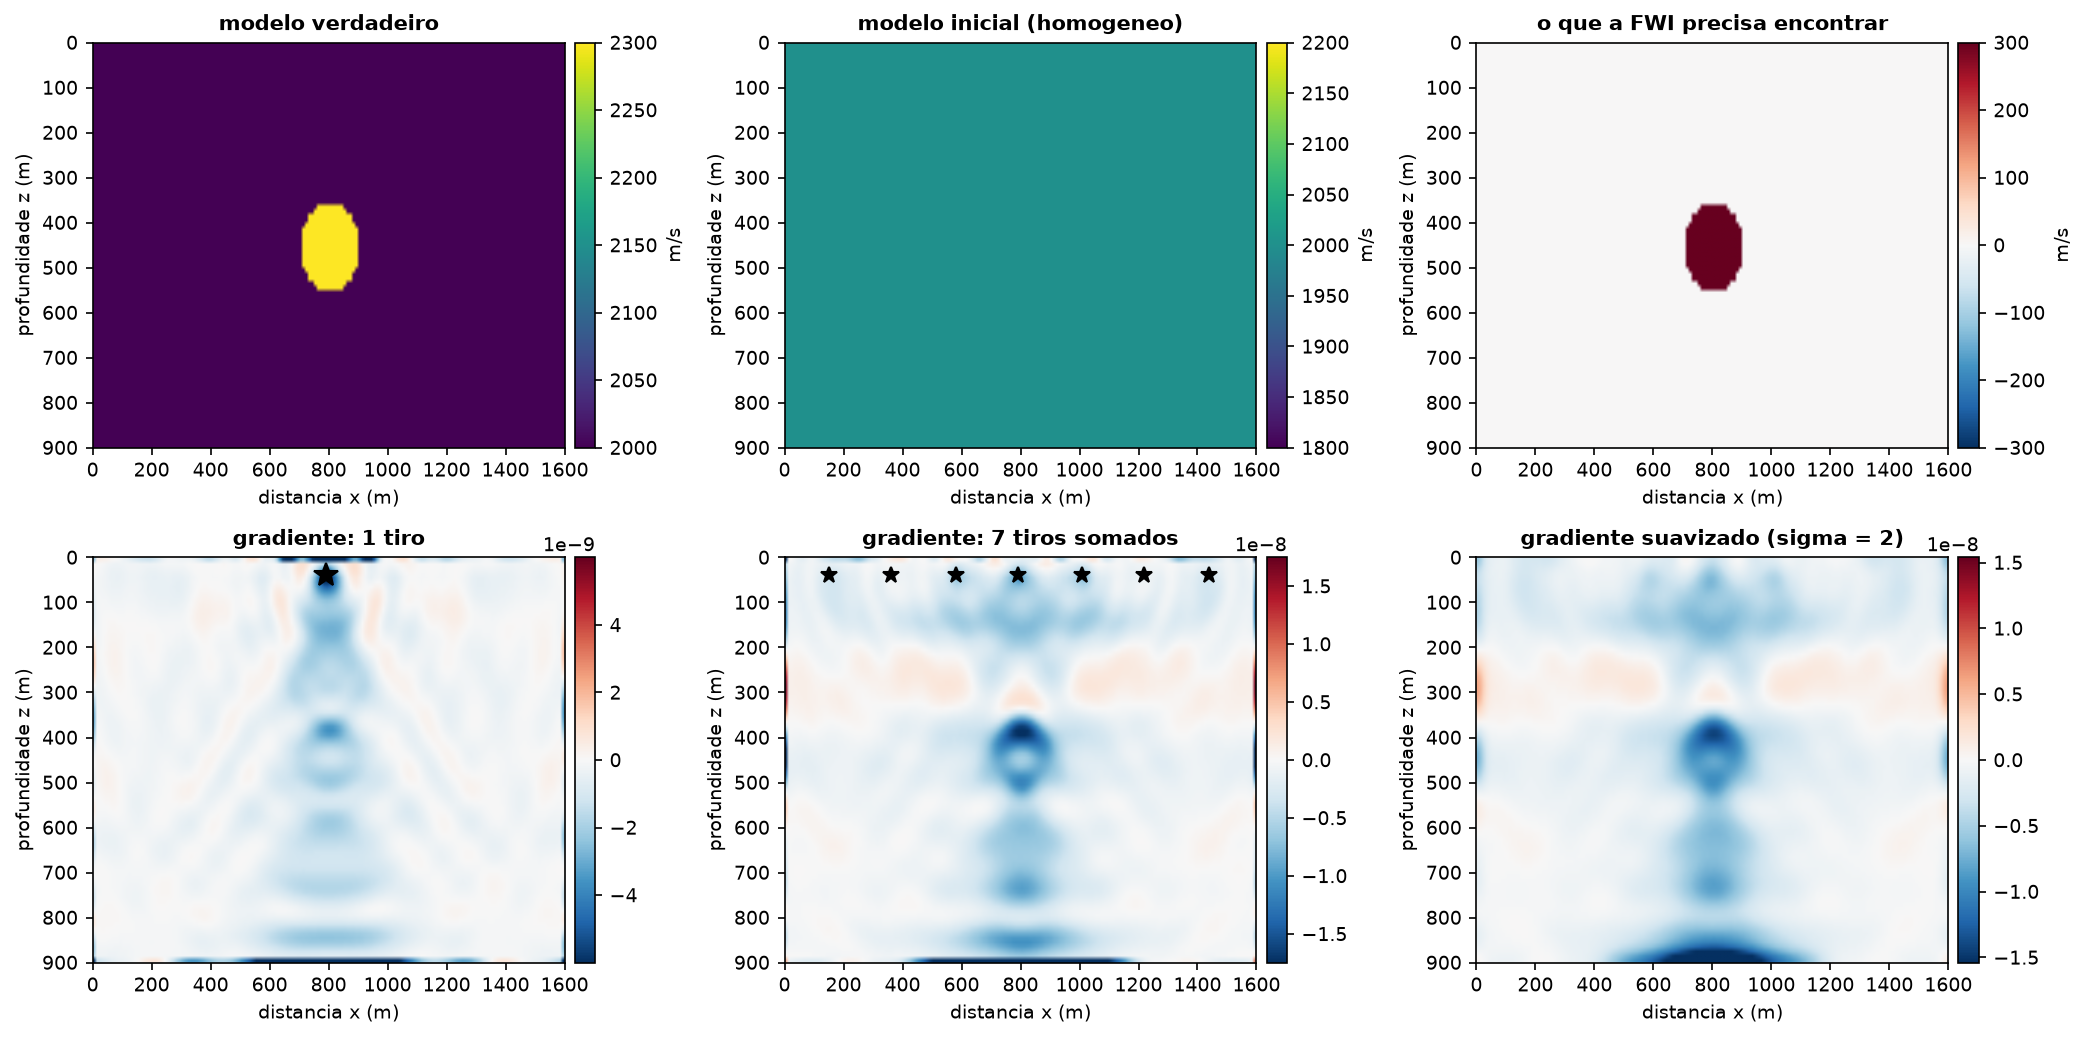
\includegraphics[width=\textwidth]{../saidas/aula08/01_gradiente_adjunto.png}
\caption{Gradiente adjunto: um tiro (esquerda, inferior), sete tiros somados
(centro) e suavizado (direita). Um tiro isolado produz arcos de Fresnel
ambíguos; a soma sobre tiros é que localiza a anomalia.}
\end{figure}

\begin{enumerate}[leftmargin=*]
\item \textbf{O sinal --- e em qual parâmetro.} A atualização é
$\mathbf{m} \leftarrow \mathbf{m} - \alpha\,\mathbf{g}$, e o sentido depende
do parâmetro em que $\mathbf{g}$ está escrito. Em \textbf{velocidade}
($g_c = \partial J/\partial c$), $g_c < 0$ faz $c$ \emph{aumentar}. Em
\textbf{vagarosidade ao quadrado} ($g_m = \partial J/\partial m$, que é a
forma em que \eqref{eq:gradiente} sai), o sentido \textbf{se inverte}: como
$dm/dc = -2/c^3 < 0$, é $g_m > 0$ que faz a velocidade aumentar. As figuras
deste capítulo mostram $g_c$. Confira sempre o sinal contra uma perturbação
conhecida: é o teste de sanidade mais barato.
\item \textbf{Artefato perto de fontes e receptores.} O campo tem amplitude
enorme ali, e a correlação explode. Não é informação: é geometria.
\item \textbf{Os arcos.} Um par fonte--receptor não aponta um ponto: espalha
a sensibilidade por uma faixa. Para ondas \emph{transmitidas} a faixa liga
fonte e receptor (a ``banana''); para ondas \emph{espalhadas} ou refletidas,
como na figura, é um arco de elipse --- a isócrona --- com focos na fonte e no
receptor, passando pelo espalhador. A espessura, nos dois casos, é a zona de
Fresnel: a onda é sensível a um \emph{volume}. Resolução finita é consequência
direta disso.
\item \textbf{Iluminação decrescente com a profundidade.} Medida com o PyFWI
neste curso: razão raso/profundo de \textbf{181$\times$}. Sem correção, a FWI
só atualiza a parte rasa.
\end{enumerate}

\section{Pré-condicionamento}

\aula{10}

\begin{teoria}[O que o pré-condicionamento realmente é]
A atualização ideal de Newton seria $\delta\mathbf{m} = -H^{-1}\mathbf{g}$, com
$H$ a Hessiana --- grande demais para ser montada. O pré-condicionador $P$ é
uma aproximação barata de $H^{-1}$.

A diagonal de $H_{GN}$ é bem \textbf{aproximada} pela energia do campo direto
em cada ponto --- a iluminação. A aproximação tem nome e referência: é o
\emph{pseudo-Hessiano} de Shin \emph{et al.} (2001), que fica só com a
diagonal (despreza o acoplamento entre pontos do modelo) e ainda despreza a
propagação de cada ponto até os receptores.

É uma aproximação, não uma identidade --- a diagonal exata de $J'^{T}J'$
envolve também essa função de Green até os receptores. Mas é boa o bastante, e
barata o bastante, para ser o pré-condicionador padrão. Dividir o gradiente
pela energia do campo, portanto, não é um truque cosmético: é uma aproximação
diagonal justificada de $H^{-1}$. É o que o PyFWI faz em
\texttt{energy\_balancing}.

O que ele \textbf{não} faz: não corrige cycle skipping, não inventa informação
onde não houve iluminação, e não substitui um bom modelo inicial.
\end{teoria}

Efeito medido (correlação do gradiente com a perturbação verdadeira):

\begin{center}
\begin{tabular}{@{}lr@{}}
\toprule
\textbf{Versão do gradiente} & \textbf{Correlação} \\
\midrule
bruto & $+0{,}0390$ \\
mascarado (superfície) & $+0{,}0830$ \\
mascarado + suavizado & $+0{,}0842$ \\
+ compensação de profundidade & $+0{,}0898$ \\
\texttt{energy\_balancing} + \texttt{g\_smooth} (PyFWI) & $+0{,}0880$ \\
\bottomrule
\end{tabular}
\end{center}

\begin{atencao}[Como ler esses valores]
Os números absolutos são baixos, e isso está \emph{certo}. Um gradiente não é
o modelo: é uma direção de busca, espalhada nos arcos de Fresnel e comparada
aqui com uma anomalia de $\sim$300 pixels em 10\,000. Esperar correlação alta
seria esperar que a FWI terminasse numa iteração.

O que importa é a variação \emph{relativa}: o tratamento mais que dobra a
correlação, e esse ganho, repetido a cada iteração, muda a convergência da
inversão inteira.
\end{atencao}

\textbf{Receita, na ordem de importância:} (1) mascare a faixa de
fonte/receptor; (2) compense a iluminação; (3) suavize
($\sigma = 1$ a $3$ células); (4) limite o modelo a uma caixa física.

% =====================================================================
\chapter{Verificação do gradiente}
\label{cap:verificacao}

\aula{09}

\section{Por que este é o teste mais importante do seu código}

\begin{armadilha}[O modo de falha silencioso]
Um gradiente errado \textbf{não} gera erro nem trava o programa. Ele gera uma
inversão que roda até o fim, produz uma curva de convergência decrescente e
devolve um modelo plausível --- e errado.

Nenhum dos sintomas normais aparece. Você só descobre quando alguém tenta
reproduzir. Por isso a verificação de gradiente é \emph{obrigatória}: é o
único teste que separa ``o código roda'' de ``o código está certo''.
\end{armadilha}

\section{Os três testes}

\subsection{Diferenças finitas pontuais}

Compara $\partial J/\partial m_i$ em alguns pixels. Serve para
\textbf{localizar} onde o gradiente erra. Resultado medido pela aula 09:

\begin{center}
\begin{tabular}{@{}lrrrr@{}}
\toprule
\textbf{Ponto} & $|g|$ relativo & \textbf{Adjunto} & \textbf{Dif.\ finitas} & \textbf{Razão} \\
\midrule
(0, 50)  & $1{,}0$              & $4{,}7484\times10^{1}$  & $4{,}7489\times10^{1}$  & 0{,}9999 \\
(17, 89) & $5{,}1\times10^{-1}$ & $-2{,}4217\times10^{1}$ & $-2{,}4219\times10^{1}$ & 0{,}9999 \\
(34, 89) & $2{,}1\times10^{-1}$ & $9{,}8459$              & $9{,}8452$              & 1{,}0001 \\
(14, 21) & $8{,}7\times10^{-2}$ & $-4{,}1222$             & $-4{,}1195$             & 1{,}0006 \\
(38, 27) & $1{,}0\times10^{-7}$ & $4{,}86\times10^{-6}$   & $4{,}28\times10^{-3}$   & 0{,}0011 \\
\bottomrule
\end{tabular}
\end{center}

A última linha é instrutiva: num ponto de gradiente desprezível, numerador e
denominador são ambos da ordem do ruído de \texttt{float32}, e a razão entre
eles não significa nada. \textbf{Isso não é erro de gradiente} --- é o limite
de precisão do próprio teste. Por isso o teste pontual serve para localizar,
nunca para aprovar ou reprovar.

\subsection{Derivada direcional}

Compara $\langle \mathbf{g}, \mathbf{h}\rangle$ com a diferença centrada ao
longo de $\mathbf{h}$. Testa o gradiente inteiro num número só, e custa 2
modelagens por $\alpha$. É o teste do dia a dia.

\begin{center}
\begin{tabular}{@{}rrr@{}}
\toprule
$\alpha$ & \textbf{Numérico (centrado)} & \textbf{Razão} \\
\midrule
0{,}4  & $4{,}56559876\times10^{-6}$ & 1{,}000661 \\
0{,}2  & $4{,}56776551\times10^{-6}$ & 1{,}000186 \\
0{,}1  & $4{,}56870921\times10^{-6}$ & 0{,}999980 \\
0{,}05 & $4{,}56812642\times10^{-6}$ & 1{,}000107 \\
0{,}02 & $4{,}57093344\times10^{-6}$ & 0{,}999493 \\
0{,}01 & $4{,}56566693\times10^{-6}$ & 1{,}000646 \\
\bottomrule
\end{tabular}
\end{center}
{\small Erro máximo: 0{,}07\%.}

\begin{pratica}[Como diagnosticar a partir do padrão]
\begin{itemize}[leftmargin=*]
\item \textbf{Razão $\approx 1$ e estável} $\Rightarrow$ gradiente correto.
\item \textbf{Razão estável mas $\ne 1$} (por exemplo 0{,}91 em todos os
$\alpha$) $\Rightarrow$ erro \textbf{sistemático}: fator de escala esquecido,
sinal trocado, peso de quadratura ($\Delta t$, $\Delta h^2$) faltando, ou
termo ausente no adjunto. Valor estável é boa notícia: o bug é determinístico.
\item \textbf{Razão instável} $\Rightarrow$ ruído numérico. Reduza a faixa de
$\alpha$ ou use precisão dupla.
\end{itemize}
\end{pratica}

\begin{atencao}[A escolha da direção $\mathbf{h}$]
Uma direção \emph{aleatória} é quase ortogonal ao gradiente (que é suave), o
que deixa $\langle\mathbf{g},\mathbf{h}\rangle$ pequeno e o teste dominado
pela curvatura. Use uma direção \textbf{suave} --- o próprio gradiente
normalizado é a escolha mais confiável.
\end{atencao}

\subsection{Teste de Taylor}

O teste definitivo: não compara valores, compara \emph{taxas de convergência}.
\begin{align}
E_0(\alpha) &= \bigl|J(\mathbf{m}+\alpha\mathbf{h}) - J(\mathbf{m})\bigr|
 \;\sim\; \mathcal{O}(\alpha), \\
E_1(\alpha) &= \bigl|J(\mathbf{m}+\alpha\mathbf{h}) - J(\mathbf{m})
 - \alpha\langle\mathbf{g},\mathbf{h}\rangle\bigr|
 \;\sim\; \mathcal{O}(\alpha^{2}).
\end{align}

\begin{center}
\begin{tabular}{@{}rrrrr@{}}
\toprule
$\alpha$ & $E_0$ & $E_1$ & ordem $E_0$ & ordem $E_1$ \\
\midrule
0{,}4   & $2{,}285\times10^{-6}$ & $4{,}578\times10^{-7}$ & --- & --- \\
0{,}2   & $1{,}028\times10^{-6}$ & $1{,}146\times10^{-7}$ & 1{,}15 & \textbf{2{,}00} \\
0{,}1   & $4{,}855\times10^{-7}$ & $2{,}867\times10^{-8}$ & 1{,}08 & \textbf{2{,}00} \\
0{,}05  & $2{,}355\times10^{-7}$ & $7{,}116\times10^{-9}$ & 1{,}04 & \textbf{2{,}01} \\
0{,}025 & $1{,}160\times10^{-7}$ & $1{,}756\times10^{-9}$ & 1{,}02 & \textbf{2{,}02} \\
\bottomrule
\end{tabular}
\end{center}

$E_0 \sim \mathcal{O}(\alpha)$ confirma que $J$ é diferenciável e que a
perturbação está no regime linear. $E_1 \sim \mathcal{O}(\alpha^{2})$ confirma
que o gradiente é \textbf{exato} --- porque só então o termo de primeira ordem
é cancelado perfeitamente e sobra a curvatura.

\textbf{Se $E_1$ cair como $\mathcal{O}(\alpha)$}, sobrou termo de primeira
ordem: o gradiente não é a derivada correta. É o diagnóstico mais informativo
de todos.

\begin{figure}[htbp]
\centering
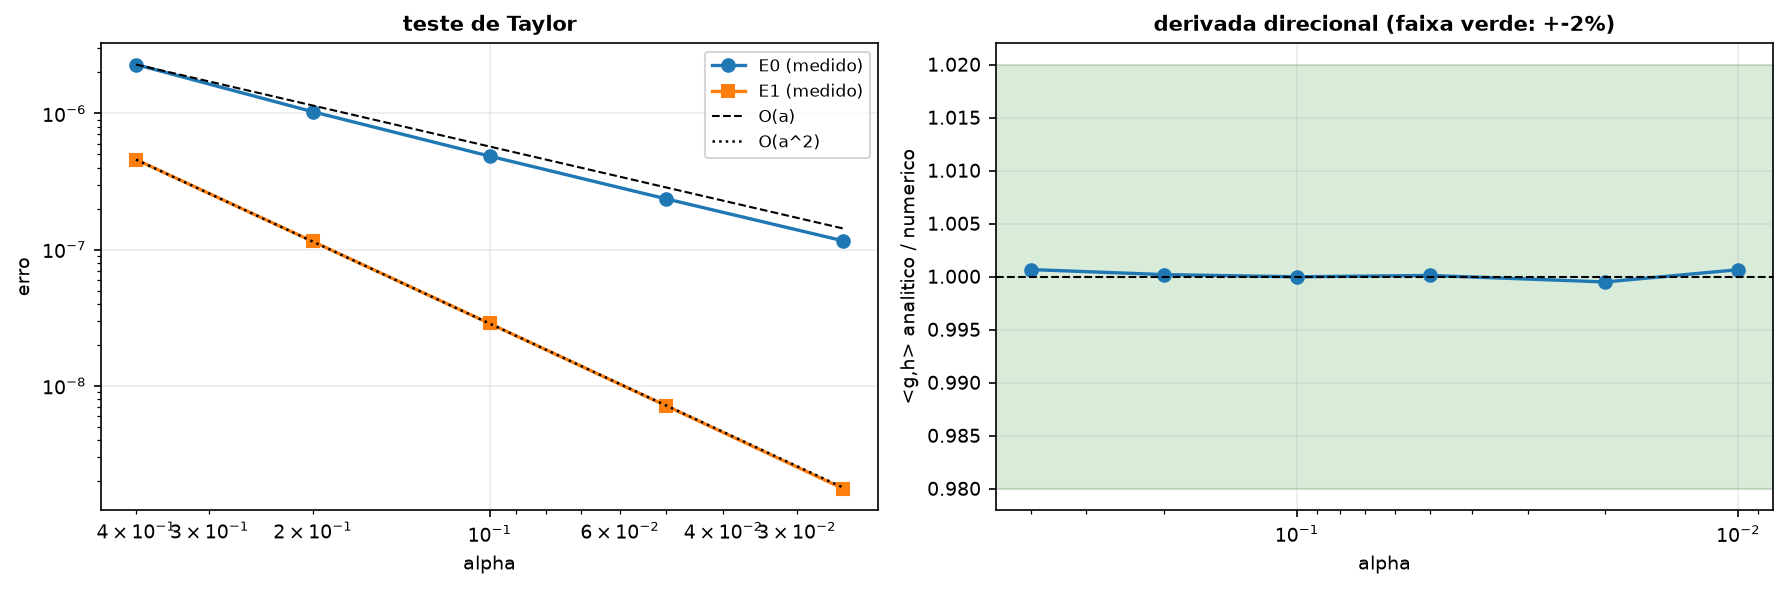
\includegraphics[width=\textwidth]{../saidas/aula09/01_testes_de_gradiente.png}
\caption{Esquerda: teste de Taylor em escala log-log, com as retas de
referência $\mathcal{O}(\alpha)$ e $\mathcal{O}(\alpha^2)$. Direita: razão da
derivada direcional (faixa verde: $\pm 2\%$).}
\end{figure}

\section{Estudo de caso: o bug que estes testes encontraram}

Vale o relato completo, porque mostra os três testes se complementando.

O propagador deste curso \textbf{reprovou} no teste da derivada direcional:

\begin{center}
\begin{tabular}{@{}rrr@{}}
\toprule
$\alpha$ & numérico & razão \\
\midrule
0{,}4  & $2{,}41766\times10^{-6}$ & 0{,}911797 \\
0{,}2  & $2{,}41808\times10^{-6}$ & 0{,}911639 \\
0{,}1  & $2{,}41747\times10^{-6}$ & 0{,}911871 \\
0{,}05 & $2{,}41784\times10^{-6}$ & 0{,}911728 \\
0{,}02 & $2{,}41946\times10^{-6}$ & 0{,}911119 \\
0{,}01 & $2{,}41739\times10^{-6}$ & 0{,}911900 \\
\bottomrule
\end{tabular}
\end{center}

O padrão é decisivo: $0{,}9118$ em \emph{todos} os $\alpha$, ao longo de uma
faixa de $40\times$. Perfeitamente estável --- o que descarta ruído numérico e
aponta para erro sistemático.

O teste \textbf{pontual} localizou a região: razões $\approx 0{,}99$ no miolo
do modelo e $\approx 0{,}72$ perto da superfície. O erro estava nas bordas.

A causa: a extensão do modelo para a moldura absorvente usa
\texttt{mode='edge'}, que replica cada pixel de borda por toda a moldura ---
operador linear $E$. O gradiente estava voltando ao domínio físico com um
simples recorte, mas $E^{T}$ não é recortar, é \textbf{somar a moldura de
volta}:

\begin{lstlisting}
# ERRADO -- descarta a sensibilidade acumulada na moldura
g_m = g_ext[topo:topo+nz, n:n+nx]

# CERTO -- E^T: dobra a moldura de volta sobre as bordas
g[topo]      += g[:topo].sum(axis=0)
g[topo+nz-1] += g[topo+nz:].sum(axis=0)
g[:, n]      += g[:, :n].sum(axis=1)
g[:, n+nx-1] += g[:, n+nx:].sum(axis=1)
\end{lstlisting}

Com a correção, a razão passou de $0{,}9118$ para $1{,}0001$.

\begin{teoria}[A lição generalizável]
\textbf{Toda operação aplicada ao modelo antes de propagar precisa do seu
adjunto no caminho de volta do gradiente}: extensão de bordas, interpolação
entre malhas, suavização, reparametrização, mudança de unidade.

Se você esqueceu de uma, o teste de gradiente acusa --- e é o único que acusa.
\end{teoria}

% =====================================================================
\part*{\centering\color{azulfwi} Parte IV --- Otimização, FWI completa e regularização}
\addcontentsline{toc}{part}{Parte IV --- Otimização, FWI completa e regularização}

\chapter{Otimização}
\label{cap:otimizacao}

\aula{11}

\section{O panorama}

Todos os métodos têm a forma \eqref{eq:iteracao}. O que muda é como se
constrói $\mathbf{d}_k$.

\begin{center}
\begin{tabular}{@{}llll@{}}
\toprule
\textbf{Método} & $\mathbf{d}_k$ & \textbf{Memória} & \textbf{Em FWI} \\
\midrule
Newton          & $-H^{-1}\mathbf{g}$ & $N^{2}$ & impossível \\
Gauss--Newton   & $-(J'^TJ')^{-1}\mathbf{g}$ & $N^{2}$ & só truncado \\
Descida máxima  & $-\mathbf{g}$ & $N$ & barato, lento \\
Grad.\ conjugado& $-\mathbf{g} + \beta\mathbf{d}_{k-1}$ & $2N$ & bom custo/benefício \\
l-BFGS          & $-H_{aprox}\mathbf{g}$ & $2mN$ & o padrão \\
\bottomrule
\end{tabular}
\end{center}

Com $N = 10^{6}$, a Hessiana tem $10^{12}$ entradas: 4\,TB em
\texttt{float32}. Não se monta, não se armazena, não se inverte.

Mas a Hessiana \emph{importa}: na diagonal, a iluminação de cada ponto; fora
da diagonal, o acoplamento entre parâmetros. Os métodos quase-Newton existem
para capturar parte disso sem montar a matriz. O l-BFGS constrói uma
aproximação da \emph{inversa} usando apenas os últimos $m$ pares
$(\mathbf{s}_k, \mathbf{y}_k)$, com $\mathbf{s}_k = \mathbf{m}_{k+1}-\mathbf{m}_k$
e $\mathbf{y}_k = \mathbf{g}_{k+1}-\mathbf{g}_k$.

\section{A busca linear, onde o tempo é gasto}

Achar a direção é metade do trabalho; decidir \emph{quanto andar} é a outra.
Em FWI cada tentativa custa uma modelagem completa de todos os tiros.

\begin{equation}
J(\mathbf{m} + \alpha\mathbf{d}) \le J(\mathbf{m})
 + c_1\,\alpha\,\langle\mathbf{g},\mathbf{d}\rangle
\qquad\text{(Armijo)}
\end{equation}

\textbf{Retrocesso:} tente $\alpha$, se falhar reduza pela metade. Gasta 5--10
avaliações. \textbf{Ajuste parabólico:} já se conhece $J(0)$ e a inclinação
$\langle\mathbf{g},\mathbf{d}\rangle$; com \emph{uma} avaliação extra fica
determinada a parábola
\[
q(\alpha) = J_0 + \langle\mathbf{g},\mathbf{d}\rangle\alpha + c\,\alpha^{2},
\qquad
\alpha^{*} = -\frac{\langle\mathbf{g},\mathbf{d}\rangle}{2c},
\]
cujo mínimo dá o passo. Acerta em $\sim$2 avaliações.

\begin{pratica}[O chute inicial do passo]
Em FWI o critério com significado físico é: \emph{não altere o modelo em mais
de 1--3\% de uma vez}. Isso é mais confiável que qualquer estimativa
puramente matemática, porque respeita a escala do problema.
\end{pratica}

\section{Comparação medida}

Problema real de FWI, malha $60\times100$, 5 tiros, $f_0 = 8$\,Hz, 12
iterações, mesmo pré-condicionamento:

\begin{center}
\begin{tabular}{@{}lrrrr@{}}
\toprule
\textbf{Método} & $J_{final}/J_0$ & \textbf{erro final} & \textbf{ganho} & \textbf{avaliações} \\
\midrule
Descida máxima      & 0{,}1035 & 3{,}82\% & $+19{,}0\%$ & 30 \\
Gradiente conjugado & 0{,}0493 & 3{,}29\% & $+30{,}1\%$ & 28 \\
l-BFGS              & 0{,}0419 & 3{,}26\% & $+30{,}7\%$ & 28 \\
\bottomrule
\end{tabular}
\end{center}
{\small (erro do modelo inicial: 4{,}71\%)}

\begin{figure}[htbp]
\centering
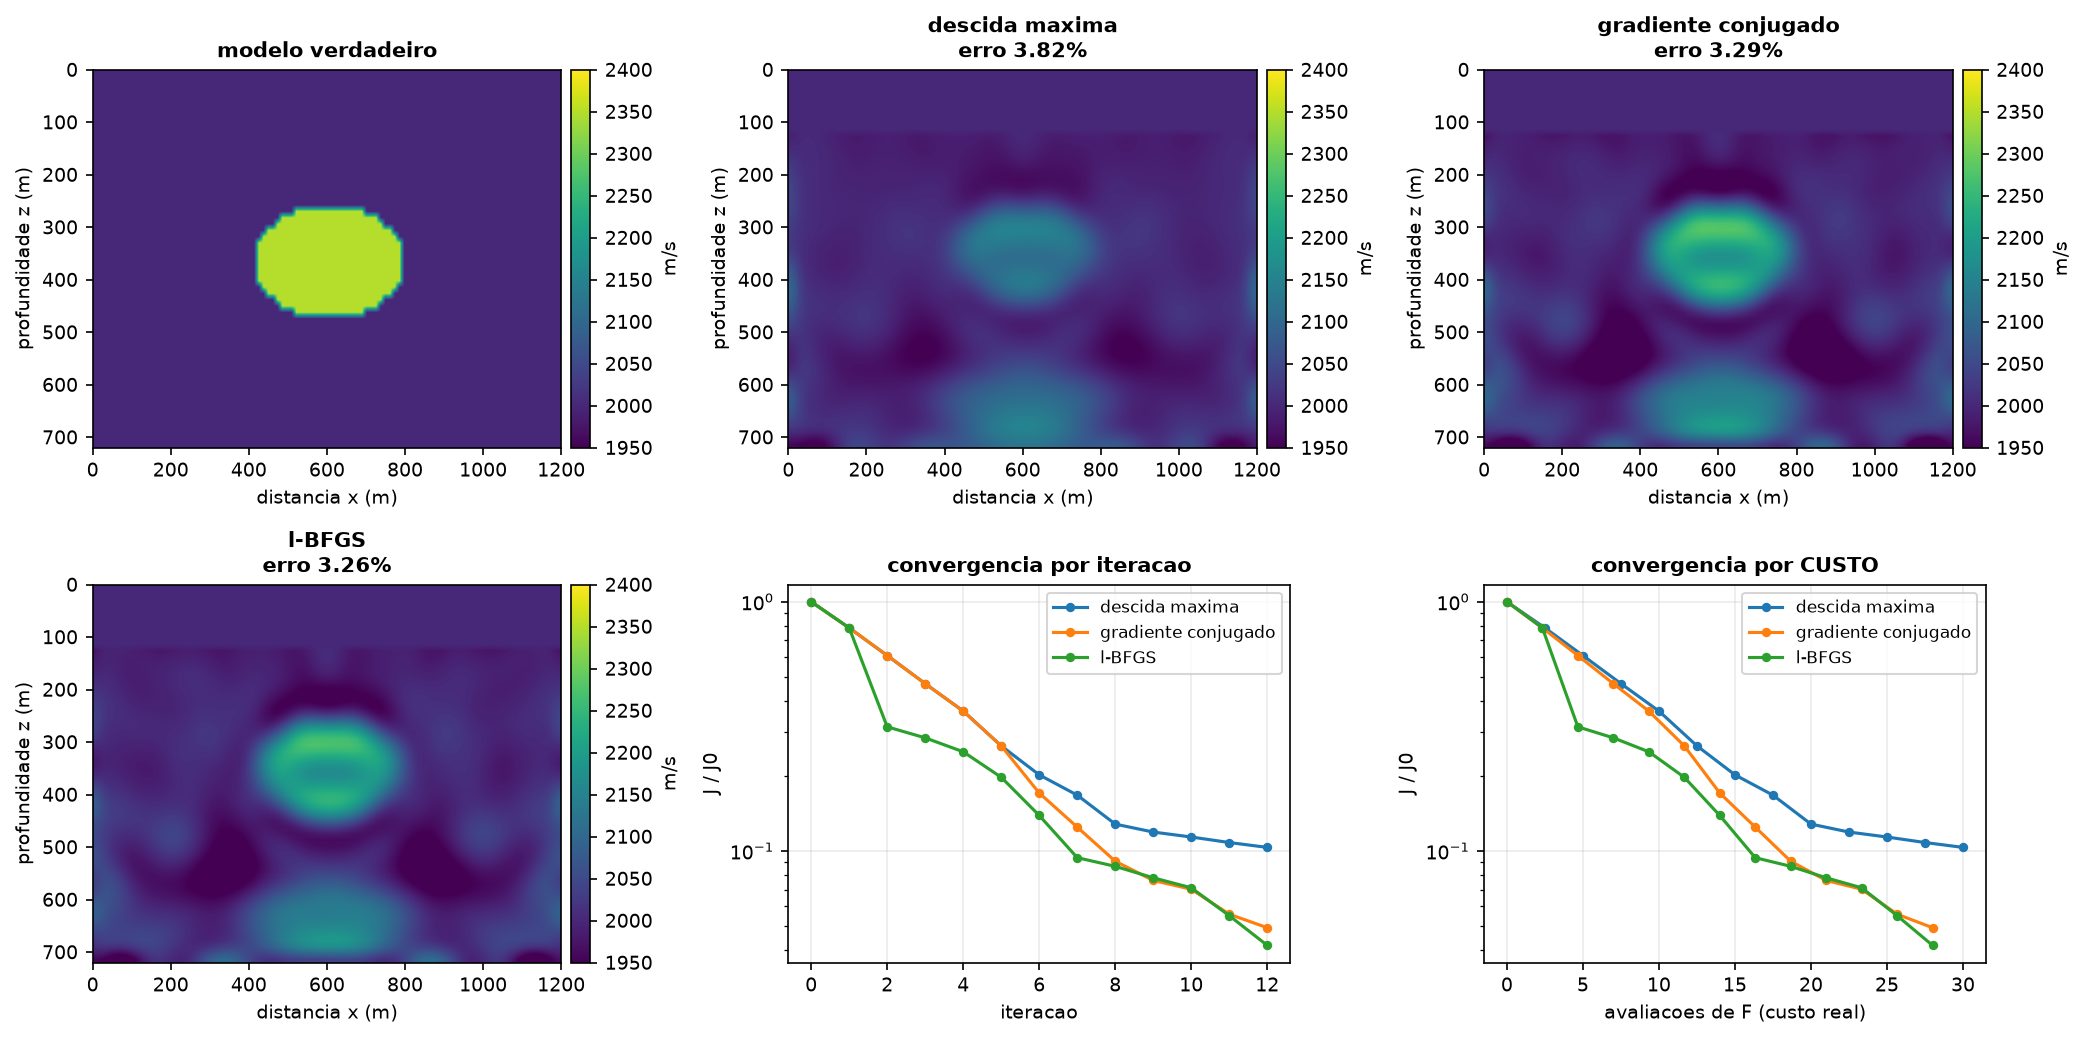
\includegraphics[width=\textwidth]{../saidas/aula11/01_comparacao_otimizadores.png}
\caption{Comparação dos três otimizadores. Os dois painéis inferiores à
direita contam histórias diferentes: por iteração e por custo.}
\end{figure}

\begin{atencao}[Compare por CUSTO, não por iteração]
Por \emph{iteração}, o l-BFGS quase sempre vence, porque cada iteração usa
curvatura acumulada. Por \emph{custo} --- número de modelagens, que é o que
consome tempo de máquina --- a comparação pode mudar, porque o número de
avaliações da busca linear varia de método para método. Neste experimento a
conta ficou praticamente empatada (30, 28 e 28 avaliações), mas não conte com
isso: um método que precise de mais tentativas por passo perde no eixo de
custo o que ganhou no de iteração.

Sempre que comparar otimizadores num relatório, mostre o eixo de custo.
Comparar por iteração favorece artificialmente os métodos de iteração cara.
\end{atencao}

\begin{pratica}[Dois detalhes que resolvem a maioria dos problemas]
\textbf{1.} \textbf{Reinicie o l-BFGS ao trocar de banda de frequência} na
multiescala. Os pares $(\mathbf{s},\mathbf{y})$ descrevem a curvatura do
problema \emph{antigo}; mantidos, atrapalham.

\textbf{2.} Se a busca linear falhar ($\alpha = 0$), não insista com mais
iterações. Quase sempre significa que a direção não é de descida ---
gradiente errado, pré-condicionamento exagerado, ou é hora de reiniciar.
\end{pratica}

% =====================================================================
\chapter{A FWI completa: multiescala}

\aula{12}

\section{A estratégia}

\begin{lstlisting}
m = m_inicial
para cada banda f em [f_baixa ... f_alta]:
    filtre d_obs com passa-baixa em f
    rode algumas iteracoes de FWI partindo de m
    m <- resultado
\end{lstlisting}

Cada banda entrega ao estágio seguinte um modelo que já está dentro do vale
de atração mais estreito da próxima. O método percorre a não convexidade em
degraus.

No PyFWI, \texttt{freqs} são as frequências de corte de um filtro Butterworth
passa-baixa aplicado a $\mathbf{d}_{obs}$ e $\mathbf{d}_{calc}$ dentro de
\texttt{cost\_seismic}; \texttt{iter} é a lista de iterações por banda. Os
parâmetros \texttt{k\_0=1, k\_end=2} restringem a atualização a $v_p$,
evitando \emph{crosstalk} com $\rho$.

\section{Um experimento controlado}

Mesmo modelo inicial, mesmo otimizador, \emph{mesmo número total de
iterações} (12). A única diferença é a ordem em que a informação entra.

\begin{center}
\begin{tabular}{@{}lrrr@{}}
\toprule
\textbf{Métrica} & \textbf{Inicial} & \textbf{Mono (25\,Hz)} & \textbf{Multi (5/12/25)} \\
\midrule
Erro relativo & 8{,}00\% & 7{,}35\% & \textbf{7{,}20\%} \\
Ganho sobre o inicial & --- & $+8{,}1\%$ & $+10{,}0\%$ \\
Correlação & 0{,}9333 & 0{,}9173 & 0{,}9296 \\
$R^{2}$ & 0{,}7284 & 0{,}7708 & \textbf{0{,}7799} \\
Tempo & --- & 3{,}8 min & 5{,}7 min \\
\bottomrule
\end{tabular}
\end{center}

Erro relativo dos dados: 0{,}2573 (inicial) $\to$ 0{,}0719 (final).

\begin{atencao}[Leia este resultado com honestidade]
A vantagem da multiescala aqui é real mas \textbf{modesta} --- 0{,}15 pontos
percentuais. E isso é esperado: o modelo inicial tem apenas 8\% de erro e
correlação 0{,}93 com o verdadeiro, ou seja, já está \emph{dentro} do vale de
atração de 25\,Hz. Quando o monoescala não sofre cycle skipping, não há muito
para o multiescala resgatar.

A expectativa é que a vantagem cresça quando o modelo inicial piora ---
\emph{desde que} a banda mais baixa ainda comece dentro do seu vale de
atração. Por isso degradar o inicial de propósito é o que realmente mede o
valor da estratégia, e a seção seguinte mostra que a expectativa nem sempre
se confirma.
\end{atencao}

\begin{figure}[htbp]
\centering
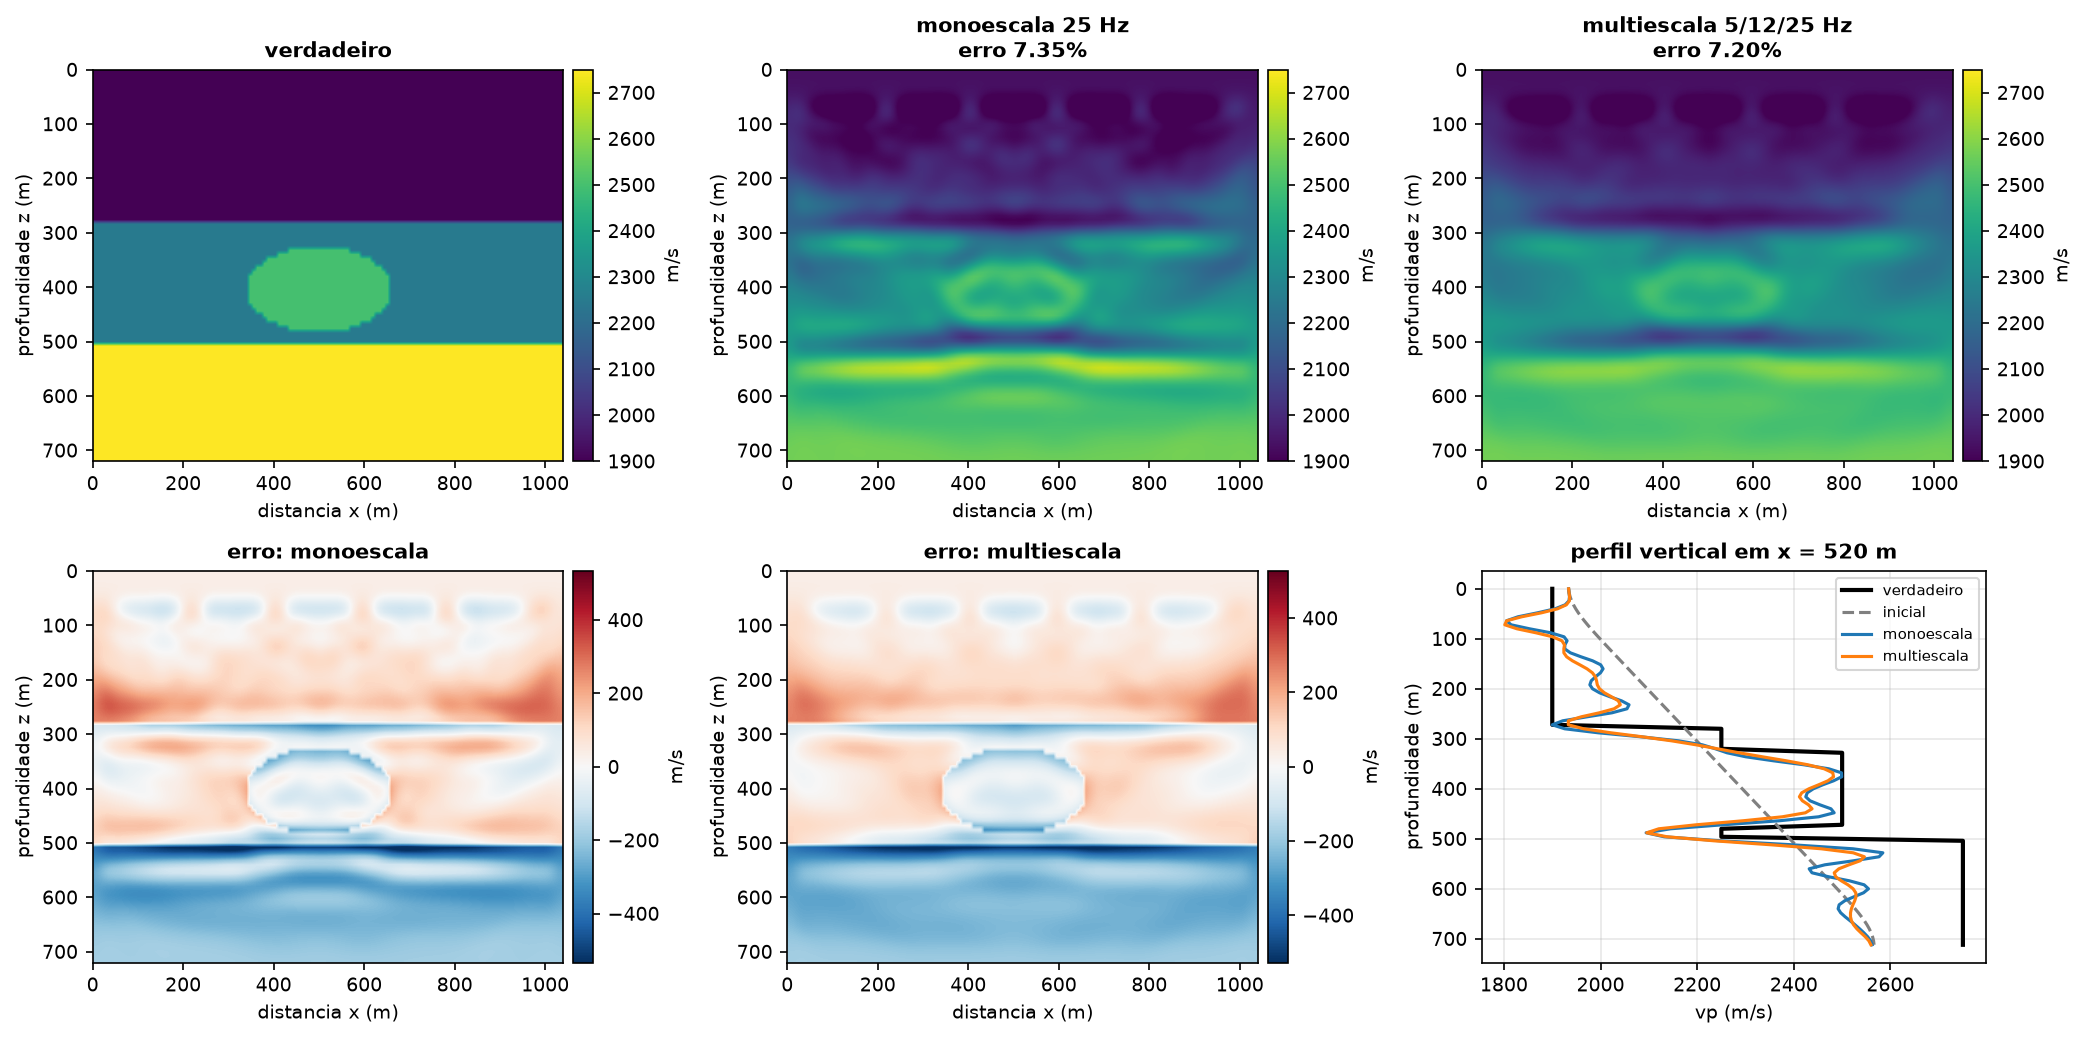
\includegraphics[width=\textwidth]{../saidas/aula12/02_mono_vs_multi.png}
\caption{Monoescala \emph{versus} multiescala: modelos recuperados, mapas de
erro e perfil vertical.}
\end{figure}

\section{Estudo de robustez: e quando o inicial é ruim?}

O experimento acima parte de um modelo inicial decente, e por isso a vantagem
da multiescala fica modesta. O teste que mede o valor real da estratégia é
degradar o inicial de propósito. Quatro modelos iniciais, com uma variante do
mesmo fluxo --- 4 tiros em vez de 6, 12 iterações no total em ambos os casos.
Os números não coincidem com os da tabela anterior: além dos tiros, o inicial
``linear suave'' não é idêntico ao de cima ($7{,}96\%$ de erro, contra
$8{,}00\%$).

\begin{center}
\begin{tabular}{@{}lrrrr@{}}
\toprule
\textbf{Modelo inicial} & \textbf{erro ini.} & \textbf{mono 25\,Hz} & \textbf{multi 5/12/25} & \textbf{vantagem} \\
\midrule
linear suave           & 7{,}96\%  & 7{,}34\%  & \textbf{7{,}07\%}  & $+0{,}27$ pp \\
linear lento (viesado) & 16{,}68\% & \textbf{17{,}57\%} & \textbf{17{,}34\%} & $+0{,}24$ pp \\
constante              & 16{,}32\% & 16{,}10\% & 16{,}06\% & $+0{,}04$ pp \\
suavizado forte        & 4{,}95\%  & 4{,}01\%  & \textbf{3{,}70\%}  & $+0{,}31$ pp \\
\bottomrule
\end{tabular}
\end{center}

\begin{teoria}[Quatro leituras, e a segunda é a mais importante]
\textbf{Primeira:} a multiescala venceu em \emph{todos} os casos. A vantagem é
consistente, ainda que modesta nesta escala de problema.

\textbf{Segunda --- olhe a linha ``linear lento''.} O erro inicial era
$16{,}68\%$ e a FWI terminou em $17{,}57\%$ (mono) e $17{,}34\%$ (multi). Ou
seja: \textbf{a inversão piorou o modelo}. Ela não travou, não deu erro, e a
função objetivo caiu direitinho. Ela simplesmente convergiu para um mínimo
local e, no caminho, degradou o que já se sabia.

Este é o fracasso mais perigoso da FWI, porque \emph{não se parece com
fracasso}. Olhando só a curva de $J$ e a figura do modelo final, você
concluiria que funcionou. É por isso que reportar o erro do modelo
\textbf{inicial} não é formalidade: sem ele, não há como saber se a inversão
ajudou.

\textbf{Terceira:} o melhor resultado absoluto ($3{,}70\%$) veio do inicial
``suavizado forte'' --- que é o modelo verdadeiro filtrado, o inicial
privilegiado que só existe em teste sintético. Compare com ``constante'', que
termina em $16\%$: a diferença entre os dois não está no algoritmo, está no
que já se sabia antes de começar.

\textbf{Quarta --- a que contraria a expectativa:} a vantagem \emph{não}
cresceu quando o inicial piorou ($+0{,}24$ e $+0{,}04$\,pp nos iniciais de
$\sim$16\%, contra $+0{,}27$ e $+0{,}31$\,pp nos bons). A multiescala só
resgata o que a banda mais \emph{baixa} alcança. Por \eqref{eq:tolerancia},
com $c \approx 2300$\,m/s e percursos de 1 a 2\,km, a tolerância a 5\,Hz fica
entre $\sim$11\% e $\sim$23\%. Um erro de $\sim$16\% está na borda desse vale,
ou fora dele, já na primeira banda --- e aí nenhuma ordem de bandas salva. O
remédio seria começar mais baixo (2--3\,Hz), o que exige dado com energia
nessas frequências.
\end{teoria}

\section{Como reportar uma FWI}

\begin{teoria}[O mínimo que sustenta uma conclusão]
Uma figura de ``antes e depois'' não sustenta nada. Reporte:
\begin{itemize}[leftmargin=*]
\item \textbf{erro relativo de modelo} $\|\mathbf{m}_{est}-\mathbf{m}_{verd}\|/\|\mathbf{m}_{verd}\|$;
\item \textbf{curva de convergência} de $J$, com eixo de \emph{custo};
\item \textbf{perfis verticais} comparando verdadeiro, inicial e invertido;
\item \textbf{mapa de erro} $\mathbf{m}_{est}-\mathbf{m}_{verd}$, que revela
\emph{onde} o método falhou;
\item \textbf{comparação de sismogramas} observado $\times$ final.
\end{itemize}

E uma exigência de honestidade: \textbf{relate o erro do modelo inicial}. Uma
FWI que sai de 2\% para 1{,}5\% não demonstra quase nada; uma que sai de 20\%
para 5\% demonstra muito. Sem o ponto de partida, o número final não
significa nada.
\end{teoria}

% =====================================================================
\chapter{Regularização}
\label{cap:regularizacao}

\aula{13}

\section{Por que regularizar}

A FWI é mal posta em dois sentidos. \textbf{Espaço nulo}: existem perturbações
que praticamente não mudam os dados --- regiões não iluminadas, estruturas
menores que $\lambda/2$, combinações de parâmetros que se cancelam.
\textbf{Amplificação de ruído}: nas direções de baixa sensibilidade, um
resíduo pequeno exige perturbação grande do modelo.

\begin{equation}
J_{total}(\mathbf{m}) = J_{dados}(\mathbf{m}) + \lambda\,R(\mathbf{m})
\end{equation}

\begin{atencao}[Uma distinção que evita confusão]
Regularização \textbf{não} melhora o ajuste dos dados: no ótimo, por
construção, $J_{dados}$ só pode ficar igual ou \emph{pior} do que sem ela. O
que ela faz é escolher, entre os muitos modelos
que ajustam os dados igualmente bem, aquele mais plausível segundo um critério
que \emph{você} definiu.

Isso significa que a escolha de $R$ é uma afirmação sobre a geologia, e
precisa ser justificada como tal.
\end{atencao}

\section{Tikhonov \emph{versus} Variação Total}

\begin{align}
R_{\text{Tikhonov}}(\mathbf{m}) &= \tfrac{1}{2}\int |\nabla m|^{2}
  \qquad\text{(norma }L_2) \\
R_{\text{TV}}(\mathbf{m}) &= \int |\nabla m|
  \qquad\qquad\ \text{(norma }L_1)
\end{align}

A troca de $L_2$ por $L_1$ parece detalhe e não é. Compare o custo de
acomodar uma variação total de 1:

\begin{center}
\begin{tabular}{@{}lrr@{}}
\toprule
 & $L_2$ & $L_1$ \\
\midrule
Um salto de 1 em um ponto & 1{,}00 & 1{,}00 \\
A mesma variação em 10 passos de 0{,}1 & \textbf{0{,}10} & 1{,}00 \\
\bottomrule
\end{tabular}
\end{center}

A $L_2$ é \emph{barata} para muitas variações pequenas e cara para um salto
grande: por isso ela \textbf{suaviza}, borrando interfaces. A $L_1$ cobra o
mesmo nos dois casos: por isso ela tolera saltos nítidos enquanto ainda pune
oscilação de ruído. Daí a TV \textbf{preservar interfaces}.

\textbf{Escolha:} alvo estratificado com contatos nítidos pede TV; variação
gradual pede Tikhonov.

\section{Um resultado que contraria a expectativa}

O experimento da aula 13 usa dado com relação sinal/ruído de \textbf{0\,dB}
(ruído com a mesma energia do sinal), 3 tiros e 18 iterações:

\begin{center}
\begin{tabular}{@{}lrr@{}}
\toprule
\textbf{Variante} & \textbf{Erro final} & \textbf{Correlação} \\
\midrule
modelo inicial                 & 4{,}75\% & 0{,}9554 \\
gradiente cru, sem regularização & 3{,}60\% & 0{,}9699 \\
gradiente cru + Tikhonov       & 4{,}42\% & 0{,}9595 \\
gradiente cru + TV             & 4{,}39\% & 0{,}9613 \\
\textbf{só suavização do gradiente} & \textbf{3{,}56\%} & \textbf{0{,}9709} \\
\bottomrule
\end{tabular}
\end{center}

\begin{teoria}[Por que a regularização explícita perdeu aqui]
O modelo inicial já é suave, e com 18 iterações a inversão não tem tempo de
gerar estrutura de alta frequência. O erro que sobra \textbf{não é rugosidade}:
é falta de \emph{contraste} --- os degraus de velocidade ainda não foram
recuperados em amplitude.

Tikhonov e TV penalizam exatamente o gradiente espacial, ou seja, penalizam o
contraste que ainda falta construir. Estão puxando na direção errada
\emph{para este problema}.

E note a última linha: apenas suavizando o gradiente, sem termo algum no
funcional, chega-se ao melhor resultado da tabela. Uma operação de uma linha.
\end{teoria}

\begin{pratica}[Regularização implícita]
Existe muita regularização em FWI que raramente é reconhecida como tal:
\begin{itemize}[leftmargin=*]
\item suavização do gradiente (o \texttt{g\_smooth} do PyFWI);
\item modelo inicial suave --- ele já restringe onde a solução pode chegar;
\item estratégia multiescala --- as bandas baixas impõem suavidade;
\item parada antecipada --- poucas iterações não produzem alta frequência;
\item projeção em caixa.
\end{itemize}

Somar regularização explícita a tudo isso frequentemente
\textbf{sobre-regulariza}. O sintoma é o desta tabela: o modelo fica mais
suave e o erro \emph{aumenta}.

A conclusão prática não é ``não use regularização'', e sim: \textbf{meça};
\textbf{diagnostique antes de escolher $R$} (se o erro residual é rugosidade,
Tikhonov/TV ajudam; se é falta de contraste ou resolução, atrapalham).
\end{pratica}

\section{Escolhendo $\lambda$}

Calibre $\lambda$ de modo que $\lambda R$ valha uma fração conhecida de
$J_{dados}$ no ponto inicial (2\%, por exemplo). Isso torna a escolha
independente de unidades e reprodutível --- muito melhor que testar potências
de 10 às cegas.

Depois refine pela \textbf{curva em L}: para vários $\lambda$, ponha
$J_{dados}$ em $x$ e $R$ em $y$, ambos em log. A curva tem forma de L, e o
$\lambda$ bom fica no \emph{cotovelo}.

\begin{armadilha}[Uma exigência de honestidade]
Em problema \emph{sintético} você conhece o modelo verdadeiro e poderia
escolher $\lambda$ pelo menor erro de modelo. Em dado \textbf{real} isso é
impossível --- você só tem $J_{dados}$ e $R$. É para isso que existe a curva
em L.

Se você reportar resultados escolhendo $\lambda$ pelo erro de modelo, diga
isso explicitamente. Caso contrário o resultado parece melhor do que seria na
prática.
\end{armadilha}

\section{Modelo a priori e vínculos}

\begin{equation}
R_{priori}(\mathbf{m}) = \tfrac{1}{2}\,\bigl\|W(\mathbf{m}-\mathbf{m}_{priori})\bigr\|^{2}
\qquad\text{(Asnaashari \emph{et al.}, 2013)}
\end{equation}

A matriz $W$ diz \emph{onde} você confia no modelo a priori. Uso clássico:
peso alto ao longo de um poço, onde há perfil sônico medido, e zero longe
dele.

\begin{center}
\begin{tabular}{@{}lll@{}}
\toprule
\textbf{Vínculo} & \textbf{Como} & \textbf{Quando} \\
\midrule
Caixa ($v_{\min}, v_{\max}$) & \texttt{clip} após cada passo & \textbf{sempre} \\
Água fixa & zerar o gradiente na lâmina d'água & dado marinho \\
Máscara de profundidade & zerar abaixo da penetração & evita artefato \\
Modelo a priori & $R = \|W(\mathbf{m}-\mathbf{m}_p)\|^{2}$ & há poço/tomografia \\
Relação entre parâmetros & vincular $v_s,\rho$ a $v_p$ & multiparâmetro \\
\bottomrule
\end{tabular}
\end{center}

A projeção em caixa parece grosseira, mas evita o modo de falha mais comum da
FWI: um passo ruim empurra a velocidade para valores não físicos, a simulação
viola o CFL e a inversão não se recupera.

\begin{atencao}[Onde clipar]
Clipe \emph{também dentro} da avaliação de $J$, e não apenas após a
atualização. A busca linear avalia $J(\mathbf{m}+\alpha\mathbf{d})$
\textbf{antes} de a projeção ser aplicada, e um passo exagerado pode estourar
a simulação ali. Este curso encontrou esse \emph{overflow} exatamente assim.
\end{atencao}

% =====================================================================
\part*{\centering\color{azulfwi} Parte V --- Os limites}
\addcontentsline{toc}{part}{Parte V --- Os limites}

\chapter{Os limites da aproximação acústica}
\label{cap:limites}

\aula{14}

\section{O inventário de hipóteses}

\begin{center}
\begin{tabular}{@{}lll@{}}
\toprule
\textbf{Hipótese} & \textbf{Onde entrou} & \textbf{Quando quebra} \\
\midrule
$\mu = 0$ & Cap.~\ref{cap:acustico} & terrestre, contrastes de $v_s$ \\
densidade constante & Cap.~\ref{cap:acustico} & contrastes de impedância \\
sem atenuação ($Q\to\infty$) & Cap.~\ref{cap:acustico} & meio dissipativo, banda larga \\
isotropia & Cap.~\ref{cap:acustico} & folhelhos, fraturas \\
2D & curso inteiro & estrutura fora do plano \\
fonte conhecida & Cap.~\ref{cap:bordas} & dado real: wavelet é estimada \\
ruído gaussiano branco & Cap.~\ref{cap:inverso} & ruído coerente, múltiplas \\
\bottomrule
\end{tabular}
\end{center}

\begin{armadilha}[O princípio que vale mais que a tabela]
\textbf{O que a FWI não consegue explicar pela física, ela explica mexendo no
modelo.}

Não existe válvula de escape. Se o dado contém um efeito que o operador não
reproduz, esse efeito entra inteiro no resíduo, e o gradiente o converte em
estrutura de velocidade. O modelo final absorve o erro de física --- e parece
um modelo, não um erro.
\end{armadilha}

\section{Limite 1: densidade e a ambiguidade da impedância}

O que controla a reflexão não é a velocidade, é a \textbf{impedância}
$Z = \rho c$, com $R = (Z_2-Z_1)/(Z_2+Z_1)$:

\begin{center}
\begin{tabular}{@{}llr@{}}
\toprule
\textbf{Meio 1} & \textbf{Meio 2} & $R$ \\
\midrule
$c=2000,\ \rho=2{,}00$ & $c=2400,\ \rho=2{,}00$ & $+0{,}0909$ \\
$c=2000,\ \rho=2{,}00$ & $c=2000,\ \rho=2{,}40$ & $+0{,}0909$ \\
$c=2000,\ \rho=2{,}00$ & $c=2400,\ \rho=1{,}67$ & $+0{,}0010$ \\
\bottomrule
\end{tabular}
\end{center}

A última linha: velocidade 20\% maior e densidade 17\% menor produzem reflexão
praticamente \textbf{nula}. Uma FWI acústica de densidade constante
interpretaria essa interface como inexistente. É o exemplo mais limpo de
ambiguidade velocidade--densidade, e a raiz do \emph{crosstalk} em inversão
multiparâmetro.

\section{Limite 2: elasticidade}

Medido no Capítulo \ref{cap:pyfwi}: a diferença entre o sismograma elástico e
o acústico tem norma comparável à do próprio dado. São ondas S e conversões
P--S. Essa energia não some do dado real: ou você a modela, ou a remove no
processamento, ou ela vai para o resíduo.

\begin{center}
\begin{tabular}{@{}llll@{}}
\toprule
\textbf{Extensão} & \textbf{Parâmetros} & \textbf{Custo} & \textbf{Resolve} \\
\midrule
Acústica & $v_p$ & 1$\times$ & cinemática P \\
Acústica + $\rho$ & $v_p,\rho$ & 1$\times$ & amplitude de reflexão \\
Viscoacústica & $v_p,Q$ & 2--4$\times$ & dissipação e dispersão \\
Elástica & $v_p,v_s,\rho$ & 3--5$\times$ & ondas S, conversões, AVO \\
Viscoelástica & $+Q_p,Q_s$ & 6--10$\times$ & tudo acima \\
Anisotrópica (VTI) & $+\epsilon,\delta$ & 2--3$\times$ & folhelhos \\
\bottomrule
\end{tabular}
\end{center}

\section{Limite 3: atenuação e o fator $Q$}

O fator de qualidade $Q$ é (aproximadamente) o número de ciclos que uma onda
percorre antes de a amplitude cair por $e^{-\pi}$. Valores típicos: água
$>1000$; rocha consolidada 100--300; sedimento não consolidado 20--50;
sedimento raso saturado ou com gás 10--30.

\begin{teoria}[Dissipação e dispersão são inseparáveis]
Este é o ponto conceitual mais importante da seção, e o mais ignorado.

Um meio que atenua de forma dependente da frequência é \textbf{obrigado} a ter
velocidade de fase dependente da frequência. A razão é \textbf{causalidade}: o
sinal não pode chegar antes de ser emitido. Formalmente, as partes real e
imaginária da resposta de um sistema causal estão ligadas pelas relações de
\textbf{Kramers--Kronig}.

Consequência prática: não adianta ``corrigir a amplitude'' de um dado atenuado
e continuar usando uma equação sem perdas. Ao atenuar, o meio também mudou a
\emph{fase} --- e a FWI é um método governado por fase. Um operador sem
dissipação está errado nas duas contas ao mesmo tempo.
\end{teoria}

\subsection*{O modelo constant-$Q$ de Kjartansson}

Entre as representações da dissipação, a de Kjartansson (1979) é a mais usada
quando se quer $Q$ aproximadamente constante na banda sísmica. Ela parte de
uma lei constitutiva de potência, e o expoente se relaciona a $Q$ por
\begin{equation}
\gamma = \frac{1}{\pi}\arctan\!\left(\frac{1}{Q}\right),
\label{eq:gamma}
\end{equation}
com velocidade de fase e amplitude dadas por
\begin{equation}
c(\omega) = c_0\left(\frac{\omega}{\omega_{ref}}\right)^{\gamma},
\qquad
A(\omega) = \exp\!\left[-\frac{\omega L}{2\,Q\,c(\omega)}\right].
\label{eq:kjartansson}
\end{equation}

\begin{atencao}[Precisão da forma usada]
O fator de atenuação em \eqref{eq:kjartansson} usa $1/(2Q)$, válido para
$Q \gg 1$. A forma exata de Kjartansson traz $\tan(\pi\gamma/2)$ no lugar. A
diferença medida é de $0{,}25\%$ em $Q=10$ e $0{,}06\%$ em $Q=20$ ---
irrelevante na faixa sísmica, mas vale saber que a expressão é uma aproximação.
\end{atencao}

No domínio do tempo, essa dependência de potência conduz a operadores de
ordem \textbf{fracionária} --- por isso a implementação viscoacústica é
substancialmente mais trabalhosa que a acústica, e costuma ser feita com
laplacianos fracionários ou com uma soma de mecanismos de relaxação (modelo
SLS).

\subsection*{O que $Q$ faz com um pulso}

Aplicando o propagador analítico \eqref{eq:kjartansson} a uma Ricker de
$f_0 = 20$\,Hz, $c_0 = 2000$\,m/s, $L = 1500$\,m:

\begin{center}
\begin{tabular}{@{}rrrr@{}}
\toprule
$Q$ & $\gamma$ & \textbf{amplitude rel.} & $f$ de pico (Hz) \\
\midrule
$10\,000$ & $3{,}2\times10^{-5}$ & 1{,}0000 & 20{,}0 \\
200 & $1{,}59\times10^{-3}$ & 0{,}7738 & 18{,}8 \\
100 & $3{,}18\times10^{-3}$ & 0{,}6008 & 17{,}8 \\
50  & $6{,}37\times10^{-3}$ & 0{,}3713 & 15{,}9 \\
20  & $1{,}59\times10^{-2}$ & 0{,}1056 & 11{,}5 \\
\bottomrule
\end{tabular}
\end{center}

Três efeitos simultâneos, nenhum presente na equação acústica: a amplitude
cai, a frequência de pico \emph{desce} (as altas são atenuadas mais), e a
velocidade de fase efetiva muda.

\begin{figure}[htbp]
\centering
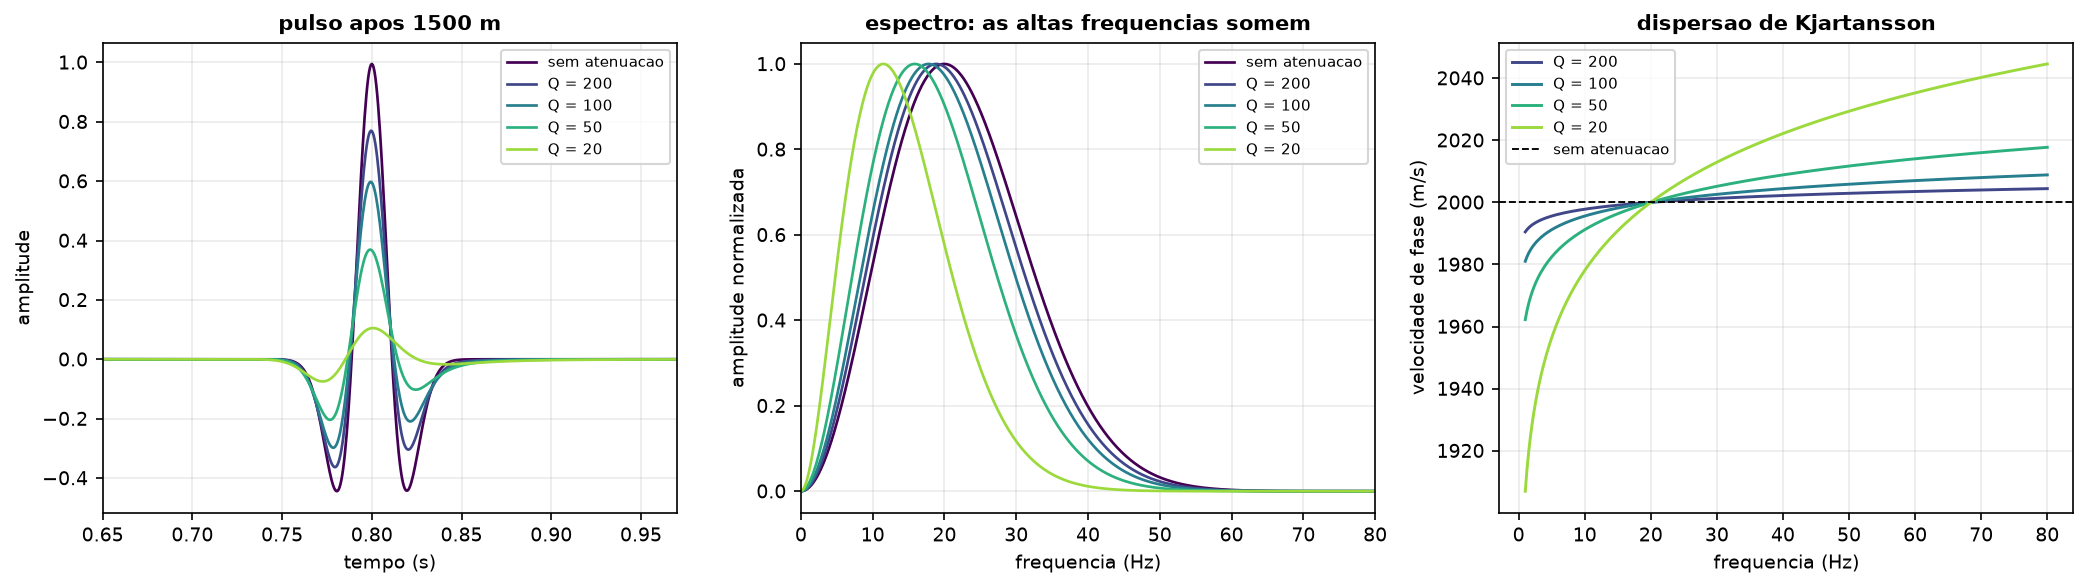
\includegraphics[width=\textwidth]{../saidas/aula14/01_atenuacao_kjartansson.png}
\caption{Efeito do modelo constant-$Q$ de Kjartansson: pulso no tempo,
espectro e dispersão da velocidade de fase.}
\end{figure}

\subsection*{Quando ignorar $Q$ provoca cycle skipping}

Aqui as peças do curso se encaixam. Modelando com $c_0$ constante mas tendo
dado de um meio dispersivo, o erro de tempo de trânsito é
\begin{equation}
\delta t(f) = \frac{L}{c_0} - \frac{L}{c(f)}
 = \frac{L}{c_0}\left[1 - \left(\frac{f}{f_{ref}}\right)^{-\gamma}\right],
\end{equation}
e o critério de meio ciclo \eqref{eq:meiociclo} decide se isso importa:

\begin{center}
\begin{tabular}{@{}rrrrrl@{}}
\toprule
$Q$ & $L$ (m) & $f$ (Hz) & $|\delta t|$ (ms) & $T/2$ (ms) & \\
\midrule
100 & 1000 & 10 & 1{,}10 & 50{,}0 & ok \\
100 & 6000 & 60 & 10{,}47 & 8{,}3 & \textbf{cycle skipping} \\
50  & 6000 & 60 & 20{,}91 & 8{,}3 & \textbf{cycle skipping} \\
20  & 1000 & 60 & 8{,}66 & 8{,}3 & \textbf{cycle skipping} \\
20  & 6000 & 10 & 33{,}25 & 50{,}0 & ok \\
10  & 6000 & 10 & 66{,}70 & 50{,}0 & \textbf{cycle skipping} \\
10  & 6000 & 60 & 102{,}76 & 8{,}3 & \textbf{cycle skipping} \\
\bottomrule
\end{tabular}
\end{center}
{\small ($c_0 = 2000$\,m/s, $f_{ref} = 20$\,Hz)}

O padrão é claro: o risco cresce com percurso \emph{longo}, frequência
\emph{alta} e $Q$ \emph{baixo}, os três juntos. Com $Q = 200$ e percursos
curtos, a aproximação sem perdas é perfeitamente defensável.

\begin{atencao}[O que a tabela não cobre]
Ela contabiliza apenas o erro de \emph{fase} por dispersão. O erro de
\emph{amplitude} por dissipação é adicional, e afeta diretamente qualquer
funcional que compare amplitudes --- como o $L_2$ usado no curso inteiro.
\end{atencao}

\section{Como decidir qual física você precisa}

A decisão se faz olhando para o dado e para o resíduo, não por gosto nem por
disponibilidade de código.

\begin{enumerate}[leftmargin=*]
\item \textbf{Olhe o resíduo}, não só o valor de $J$. Resíduo com estrutura
\emph{coerente} é a assinatura de física faltando. Resíduo que parece ruído
aleatório significa que você chegou ao limite do dado.
\item \textbf{Compare espectros} de observado e sintético em função do
\emph{offset}. Se o sintético mantém alta frequência que o dado real já perdeu
em \emph{offsets} longos, há atenuação não modelada.
\item \textbf{Verifique amplitude $\times$ offset.} Decaimento mais rápido no
dado real aponta para dissipação ou espalhamento.
\item \textbf{Procure eventos ausentes.} Energia no dado real em tempos onde o
sintético acústico não produz nada: ondas S, conversões ou múltiplas.
\item \textbf{Teste a sensibilidade.} Gere dado sintético com a física mais
completa e inverta com a mais simples. O erro de modelo resultante é a medida
direta do custo da aproximação --- e o experimento mais informativo que existe
para justificar (ou dispensar) uma extensão.
\end{enumerate}

\begin{armadilha}[O caminho inverso também tem custo]
Adicionar física sem necessidade traz mais parâmetros, mais \emph{crosstalk},
mais mínimos locais, mais tempo de máquina, e mais dificuldade em atribuir um
resultado a uma causa.

Uma FWI acústica bem feita, com bom modelo inicial e multiescala honesta,
costuma render mais que uma viscoelástica mal condicionada. A pergunta certa
não é ``qual a física mais completa?'', e sim \textbf{``qual é a física mais
simples que explica o meu dado?''}
\end{armadilha}

% =====================================================================
\appendix

\chapter{Checklist de diagnóstico}

\section*{A FWI não converge ($J$ não cai)}
\begin{enumerate}[leftmargin=*]
\item O gradiente está correto? Rode o teste de Taylor
(Cap.~\ref{cap:verificacao}). \textbf{Antes de qualquer outra coisa.}
\item A busca linear está retornando $\alpha = 0$? Direção não é de descida.
\item O sinal do gradiente está certo? Compare $-\mathbf{g}$ com uma
perturbação conhecida.
\item O passo inicial é razoável? Deve alterar o modelo em 1--3\%.
\end{enumerate}

\section*{$J$ cai mas o modelo está errado}
\begin{enumerate}[leftmargin=*]
\item \textbf{Cycle skipping.} Recomece de uma frequência mais baixa. Se o
resultado mudar, era isso.
\item Modelo inicial fora do vale de atração --- verifique com
\eqref{eq:tolerancia}.
\item Física faltando: o resíduo final tem estrutura coerente?
\item Bordas: artefatos de reflexão entrando no resíduo.
\end{enumerate}

\section*{Só a parte rasa é atualizada}
\begin{enumerate}[leftmargin=*]
\item Falta máscara na faixa de fonte/receptor.
\item Falta compensação de iluminação (\texttt{energy\_balancing}).
\item \emph{Offset} insuficiente para a profundidade desejada.
\end{enumerate}

\section*{O campo estoura (\texttt{NaN})}
\begin{enumerate}[leftmargin=*]
\item CFL: $c_{\max}\Delta t/\Delta h$ acima do limite.
\item O modelo saiu da caixa física durante a busca linear --- clipe também
\emph{dentro} da avaliação de $J$.
\end{enumerate}

\section*{Cauda oscilatória onde não deveria haver evento}
\begin{enumerate}[leftmargin=*]
\item Dispersão numérica: $G$ insuficiente. Reduza $\Delta h$, aumente a ordem
espacial, ou baixe $f_0$.
\end{enumerate}

\chapter{Notação}

\begin{center}
\begin{longtable}{@{}ll@{}}
\toprule
\textbf{Símbolo} & \textbf{Significado} \\
\midrule
\endhead
$\mathbf{m}$ & vetor de parâmetros do modelo \\
$m = 1/c^{2}$ & vagarosidade ao quadrado (parâmetro de inversão) \\
$c$, $v_p$ & velocidade de onda P (m/s) \\
$v_s$ & velocidade de onda S (m/s) \\
$\rho$ & densidade \\
$\lambda, \mu$ & parâmetros de Lamé ($\mu$ = módulo de cisalhamento) \\
$K$ & módulo de compressibilidade \\
$p$ & pressão \\
$\sigma_{ij}$ & tensor de tensões \\
$F$ & operador de modelagem direta \\
$J$ & funcional objetivo \\
$\mathbf{r}$ & vetor residual \\
$\mathbf{g}$ & gradiente \\
$H$ & Hessiana \\
$\lambda(\mathbf{x},t)$ & campo adjunto (multiplicador de Lagrange) \\
$\alpha$ & comprimento do passo \\
$\Delta h$, $\Delta t$ & espaçamento da malha e passo de tempo \\
$C$ & número de Courant \\
$G$ & pontos por comprimento de onda \\
$f_0$ & frequência de pico da fonte \\
$Q$ & fator de qualidade \\
$\gamma$ & expoente de Kjartansson \\
\bottomrule
\end{longtable}
\end{center}

\chapter{Referências}

\begin{enumerate}[leftmargin=*,itemsep=3pt]
\item ASNAASHARI, A.; BROSSIER, R.; GARAMBOIS, S.; AUDEBERT, F.; THORE, P.;
VIRIEUX, J.
\emph{Regularized seismic full waveform inversion with prior model
information.} Geophysics, v.~78, n.~2, p.~R25--R36, 2013.

\item BUNKS, C.; SALECK, F.~M.; ZALESKI, S.; CHAVENT, G.
\emph{Multiscale seismic waveform inversion.} Geophysics, v.~60, n.~5,
p.~1457--1473, 1995.

\item CARCIONE, J.~M. \emph{Wave Fields in Real Media: Wave Propagation in
Anisotropic, Anelastic, Porous and Electromagnetic Media.} 4.~ed. Elsevier,
2022.

\item CERJAN, C.; KOSLOFF, D.; KOSLOFF, R.; RESHEF, M. \emph{A nonreflecting
boundary condition for discrete acoustic and elastic wave equations.}
Geophysics, v.~50, n.~4, p.~705--708, 1985.

\item KJARTANSSON, E. \emph{Constant-Q wave propagation and attenuation.}
Journal of Geophysical Research, v.~84, p.~4737--4748, 1979.

\item LOUBOUTIN, M. \emph{et al.} \emph{Devito (v3.1.0): an embedded
domain-specific language for finite differences and geophysical exploration.}
Geoscientific Model Development, v.~12, n.~3, p.~1165--1187, 2019.

\item MARDAN, A.; GIROUX, B.; FABIEN-OUELLET, G. \emph{PyFWI: A Python package
for full-waveform inversion and reservoir monitoring.} SoftwareX, v.~22,
art.~101384, 2023.

\item MORGAN, J. \emph{et al.} \emph{Next-generation seismic experiments:
wide-angle, multi-azimuth, three-dimensional, full-waveform inversion.}
Geophysical Journal International, v.~195, n.~3, p.~1657--1678, 2013.

\item NOCEDAL, J.; WRIGHT, S.~J. \emph{Numerical Optimization.} 2.~ed.
Springer, 2006.

\item PLESSIX, R.-E. \emph{A review of the adjoint-state method for computing
the gradient of a functional with geophysical applications.} Geophysical
Journal International, v.~167, n.~2, p.~495--503, 2006.

\item SHIN, C.; JANG, S.; MIN, D.-J. \emph{Improved amplitude preservation for
prestack depth migration by inverse scattering theory.} Geophysical
Prospecting, v.~49, n.~5, p.~592--606, 2001.

\item TARANTOLA, A. \emph{Inversion of seismic reflection data in the acoustic
approximation.} Geophysics, v.~49, n.~8, p.~1259--1266, 1984.

\item VIRIEUX, J.; OPERTO, S. \emph{An overview of full-waveform inversion in
exploration geophysics.} Geophysics, v.~74, n.~6, p.~WCC1--WCC26, 2009.

\item VIRIEUX, J.; ASNAASHARI, A.; BROSSIER, R.; MÉTIVIER, L.; RIBODETTI, A.;
ZHOU, W. \emph{An introduction to full waveform inversion.} In:
\emph{Encyclopedia of Exploration Geophysics}. Tulsa: Society of Exploration
Geophysicists, 2014. p.~R1-1--R1-40. DOI 10.1190/1.9781560803027.entry6.
\end{enumerate}

\vfill
\begin{center}
{\color{cianofwi}\rule{0.55\textwidth}{1pt}}\\[0.35cm]
{\small Material gerado a partir do código em \arq{aulas/} e \arq{fwikit/}.\\
Todos os números e figuras são reprodutíveis executando as aulas.}
\end{center}

\end{document}
